 \documentclass[a4paper,12pt]{report}
\usepackage{a4wide}

%\documentclass[a5paper,10pt]{book}
%\usepackage[top=23mm, bottom=18mm, left=15mm, right=25mm]{geometry}
%\geometry{papersize={170mm,220mm}}


\usepackage[utf8x]{inputenc}
\usepackage[danish]{babel}

\usepackage{xr-hyper} %Externe hyper-ref
\usepackage[colorlinks=true, hyperindex=true, linkcolor=minmblaa, citecolor=minmblaa, urlcolor=minmblaa]{hyperref}
\hypersetup{colorlinks=true,filecolor=minmblaa,bookmarksnumbered=true} %Til hyperreferencer. Referencer med farver
\usepackage{needspace} % giver mulighed for at kræve at der skal være et antal tomme linier på siden før ellers indsættes et sideskift.
\usepackage{framed} %Bokse
\usepackage{wrapfig}

\usepackage{amsmath,amsfonts,amssymb,amsthm,mathtools} %Matematikpakker

\setlength{\parindent}{0mm} %Ingen Indhak i første linje i afsnit

\usepackage{color} %Farvepakke

\usepackage{array}
\usepackage{colortbl}
\usepackage{multirow} %Til at flette rækker i tabeller.

\usepackage{verbatim,mhchem}



	% DOWNLOAD FRA: http://sarovar.org/frs/?group_id=52&release_id=97
	% Læg i directory for hoved TEX fil
%\usepackage[draft]{pdfdraftcopy}
%\draftstring{Licens: Kasper Langt Mellemnavn Skårhøj}
%\draftfontsize{30}
	%\draftfontfamily{hlh}
	%\draftangle{45}
	%\definecolor{mycolor}{rgb}{.825,.855,1}
	%\draftcolor{mycolor}
	%\draftfontattrib



% = Sidehoved =
\usepackage{fancyhdr}
\pagestyle{fancy}
\renewcommand{\sectionmark}[1]{\markright{\protect\titlegraphic{dturoed}\textcolor{dtugraa}{\thesection~\MakeUppercase{#1}}}} % \thesection.\
\fancyhead{}
\fancyfoot{}
\fancyhead[R]{\titlefont\thepage}
\fancyhead[C]{}
\fancyhead[L]{\titlefont \small eNote \MakeUppercase{~\thechapter}~\hspace*{1ex}\rightmark}
\renewcommand\headrulewidth{0pt}
\fancypagestyle{plain}{\fancyfoot[C]{}}% {\titlefont\footnotesize\thepage}}
\setlength{\headheight}{15pt}


% = Længder
%\newlength{\envtblsep}\setlength{\envtblsep}{1\FrameSep}
\newlength{\obsl}\setlength{\obsl}{\textwidth-1.2cm-13.2pt}

% Includes:

% =     Fonts (select one)    =
\usepackage{mathpazo}\linespread{1.05} % Palatino needs more leading (space between lines)
\usepackage{bm} % bold math, must be loaded after the fontpackages

% % Til overskrifter
\DeclareTextFontCommand{\th}{\fontencoding{T1}\fontfamily{phv}\fontseries{b}\selectfont}
\newcommand\titlefont{\fontencoding{T1}\fontfamily{phv}\selectfont}


% =     PGF grafik      =
\usepackage{tikz}
\newcommand\titlegraphic[1]{%
\tikz[baseline] %
\draw[thick,color=#1]
(0pt  ,-0.25em) -- (0pt  ,0.85em)
(2.5pt,-0.25em) -- (2.5pt,0.85em)
(5pt  ,-0.25em) -- (5pt  ,0.85em)
(7.5pt,-0.25em) -- (7.5pt,0.85em);\hspace*{0.8ex} %
}

\newcommand\titlegraphicwide[1]{%
\tikz[baseline] %
\draw[line width=0.8mm,color=#1]
(0pt  ,-0.25em) -- (0pt  ,0.85em)
(4.5pt,-0.25em) -- (4.5pt,0.85em)
(9pt  ,-0.25em) -- (9pt  ,0.85em)
(13.5pt,-0.25em) -- (13.5pt,0.85em);\hspace*{0.8ex} %
}


% =      Title Layout      =
\usepackage{titlesec}
\makeatletter
\titleformat{\chapter}
	[display] % Shape
	{\titlefont\Huge\flushleft} % Title and label format
	{\titlefont\LARGE\bfseries \titlegraphicwide{dturoed}\textcolor{dtugraa}{\@chapapp~\thechapter}} % label
	{0.9em} % label/title separation
	{} % before code
	[] % after code
\makeatother
\titleformat{\section}
	[hang] % Shape
	{\titlefont\Large\flushleft} % Title and label format
	{\thesection} % label
	{0.9em} % label/title separation
	{} % before code
	[] % after code
\titleformat{\subsection}
	[hang] % Shape
	{\titlefont\large} % Title and label format
	{\thesubsection} % label
	{0.9em} % label/title separation
	{} % before code
	[] % after code
\titlespacing{\subsection}{0pt}{*6}{*1.5}
\titleformat{\subsubsection}
	[hang] % Shape
	{\titlefont} % Title and label format
	{\thesubsubsection} % label
	{0.9em} % label/title separation
	{} % before code
	[] % after code



% = Farver
\definecolor{dturoed}{rgb}{0.6, 0.0, 0.0}
\definecolor{dtugraa}{rgb}{0.5, 0.5, 0.5}	% Lidt mørkere. Korrekt = 0.4
\definecolor{mingroenstreg}{rgb}{0.4,0.8,0}	% Sekundærfarve 14 : 102/204/0	(Forårsgrøn) -> Eksempler
\definecolor{mingroen}{rgb}{0.32,0.64,0}		% Sekundærfarve 14, 80% mørkere (tekst)
\definecolor{minorangestreg}{rgb}{1,0.6,0}		% Sekundærfarve 1 : 255/153/0	(Orange) -> Opgaver
\definecolor{minorange}{rgb}{0.8,0.48,0}		% Sekundærfarve 1 , 80% mørkere (tekst)

\definecolor{minblaa}{rgb}{0.2,0.4,0.8}	% Sekundærfarve 13 , 51/102/204 	( Blå -> Definitioner etc)
\definecolor{minmblaa}{rgb}{0.16,0.32,0.64}	% Sekundærfarve 13 , 80% mørkere (tekst)
\definecolor{thmbackground}{rgb}{0.97,.97, 0.99}	% Farve 13 - lys baggrund

\definecolor{mingraastreg}{rgb}{.5,.5,.5}
\definecolor{hvadbackground}{rgb}{0.97,.97, 0.97}
\definecolor{sumgul}{rgb}{1,1,.8}

\definecolor{hjmopgfarve}{rgb}{.96,1,.96}


% = Counter
\newcounter{evncount}[chapter]
\setcounter{evncount}{0}
\renewcommand{\theevncount}{\thechapter.\arabic{evncount}}
\renewcommand{\theequation}{\thechapter-\arabic{equation}}


% = Eksempler = example =
\newenvironment{example}[1][]{
	\refstepcounter{evncount}
	\setlength{\obsl}{\textwidth-1.2cm-13.2pt-9pt} % fix width of the info envirnment%
	\def\FrameCommand{ 
		\textcolor{mingroenstreg}{\vrule width 4pt} 
		\hspace{5pt} 
	}%
	\MakeFramed{\advance\hsize-\width \FrameRestore}%
	\needspace{3\baselineskip}
	\titlegraphic{mingroen}
	\textcolor{mingroen}{
		\th{Eksempel \theevncount \hspace*{5mm} #1}
	} 
	\vspace*{3mm}%
	\begin{small}
	\par
}
{
	\end{small}
	\endMakeFramed
}


% = Opgaver = exercise =
\newenvironment{exercise}[1][]{
	\refstepcounter{evncount}
	\setlength{\obsl}{\textwidth-1.2cm-13.2pt-9pt}% fix width of the info envirnment%
	\def\FrameCommand{
		\textcolor{minorangestreg}{\vrule width 4pt}
		\hspace{5pt}
	}%
	\MakeFramed{\advance\hsize-\width \FrameRestore}%
	\needspace{3\baselineskip}
	\titlegraphic{minorange}
	\textcolor{minorange}{
		\th{Opgave \theevncount \hspace*{5mm} #1}
	} 
	\vspace*{3mm}%
	\begin{small}
	\par
}
{
	\end{small}
	\endMakeFramed
}


% = Bevis
\newenvironment{bevis}{
	\setlength{\obsl}{\textwidth-1.2cm-13.2pt-9pt} % fix width of the info envirnment%
	\def\FrameCommand{
		\textcolor{mingraastreg}{\vrule width 4pt} 
		\hspace{5pt}
	}%
	\MakeFramed{\advance\hsize-\width \FrameRestore}%
	\needspace{3\baselineskip}
	\titlegraphic{black}
	\textcolor{black}{
		\th{Bevis}
	}
	\vspace*{3mm}%
	\begin{small}
	\par
}
{
	\bevisslut 
	\end{small}
	\endMakeFramed
}


% = Definition =
\newenvironment{definition}[1][]{
	\vspace{4mm}
	\pagebreak[1]
	\setlength{\obsl}{\textwidth-1.2cm-2\FrameSep-13.2pt}%
	\def\FrameCommand{
		\fboxsep=\FrameSep\fcolorbox{minblaa}{thmbackground}
	}
	\begin{minipage}{\textwidth}
	\MakeFramed{\advance\hsize-\width\FrameRestore}
	\refstepcounter{evncount}
	\titlegraphic{minblaa}
	\textcolor{minmblaa}{
		\th{Definition \theevncount \hspace*{5mm} #1}
	}
	\vspace*{3mm}
	\par
}
{
	\endMakeFramed 
	\end{minipage}
	\vspace{4mm}
}


% = Theorem =
\newenvironment{theorem}[1][]{
	\vspace{4mm}
	\pagebreak[1]%
	\setlength{\obsl}{\textwidth-1.2cm-2\FrameSep-13.2pt}%
	\def\FrameCommand{
		\fboxsep=\FrameSep\fcolorbox{minblaa}{thmbackground}
	}%
	\begin{minipage}{\textwidth}
	\MakeFramed{\advance\hsize-\width\FrameRestore}%
	\refstepcounter{evncount}
	\titlegraphic{minblaa}
	\textcolor{minmblaa}{
		\th{Sætning \theevncount \hspace*{5mm} #1}
	}
	\vspace*{3mm}
	\par
}
{
	\endMakeFramed 
	\end{minipage}
	\vspace{4mm}
}


% = Lemma =
\newenvironment{lemma}[1][]{
	\vspace{4mm}
	\pagebreak[1]
	\setlength{\obsl}{\textwidth-1.2cm-2\FrameSep-13.2pt}%
	\def\FrameCommand{
		\fboxsep=\FrameSep \fcolorbox{minblaa}{thmbackground}
	}
	\begin{minipage}{\textwidth} 
	\MakeFramed{\advance\hsize-\width \FrameRestore}
	\refstepcounter{evncount}
	\titlegraphic{minblaa}
	\textcolor{minmblaa}{
		\th{Hjælpesætning \theevncount \hspace*{5mm} #1}
	}
	\vspace*{3mm}
	\par
}
{
	\endMakeFramed 
	\end{minipage}
	\vspace{4mm}
}


% = Corollary =
\newenvironment{corollary}[1][]{
	\vspace{4mm}
	\pagebreak[1]
	\setlength{\obsl}{\textwidth-1.2cm-2\FrameSep-13.2pt}%
	\def\FrameCommand{
		\fboxsep=\FrameSep \fcolorbox{minblaa}{thmbackground}
	}
	\begin{minipage}{\textwidth} 
	\MakeFramed{\advance\hsize-\width \FrameRestore}
	\refstepcounter{evncount}
	\titlegraphic{minblaa}
	\textcolor{minmblaa}{
		\th{Følgesætning \theevncount \hspace*{5mm} #1}
	}
	\vspace*{3mm}
	\par
}
{
	\endMakeFramed 
	\end{minipage}
	\vspace{4mm}
}


% = Metode = method
\newenvironment{method}[1][]{
	\vspace{4mm}
	\pagebreak[1]
	\setlength{\obsl}{\textwidth-1.2cm-2\FrameSep-13.2pt}%
	\def\FrameCommand{
		\fboxsep=\FrameSep \fcolorbox{black}{hvadbackground}
	}
	\begin{minipage}{\textwidth} 
	\MakeFramed{\advance\hsize-\width \FrameRestore}
	\refstepcounter{evncount}
	\titlegraphic{black}
	\textcolor{black}{
		\th{Metode \theevncount \hspace*{5mm} #1}
	}
	\vspace*{3mm}
	\par
}
{
	\endMakeFramed
	\end{minipage}
	\vspace{4mm}
}


% = Forklaring = explain =
\newenvironment{explain}[1][]{
	\vspace{4mm}
	\pagebreak[1]
	\setlength{\obsl}{\textwidth-1.2cm-2\FrameSep-13.2pt}%
	\def\FrameCommand{
		\fboxsep=\FrameSep \fcolorbox{black}{hvadbackground}
	}
	\MakeFramed{\advance\hsize-\width \FrameRestore}
	\refstepcounter{evncount}
	\titlegraphic{black}
	\textcolor{black}{
		\th{Forklaring \theevncount \hspace*{5mm} #1}
	}
	\vspace*{3mm}
	\par
}
{
	\endMakeFramed
	\vspace{4mm}
}


% = Bemærkning = remark =
\newenvironment{remark}[1][]{
	\vspace{4mm}
	\pagebreak[1]
	\setlength{\obsl}{\textwidth-1.2cm-2\FrameSep-13.2pt}%
	\def\FrameCommand{
		\fboxsep=\FrameSep \fcolorbox{black}{hvadbackground}
	}
	\begin{minipage}{\textwidth} 
	\MakeFramed{\advance\hsize-\width \FrameRestore}
	\refstepcounter{evncount}
	\titlegraphic{black}
	\textcolor{black}{
		\th{Bemærkning \theevncount \hspace*{5mm} #1}
	}
	\vspace*{3mm}
	\par
}
{
	\endMakeFramed 
	\end{minipage}
	\vspace{4mm}
}







% = OBS! = obs =
\newenvironment{obs}{\vspace{4mm}\par%
\begin{tabular}{m{1.2cm}<{\hspace*{2mm}}@{}|m{\obsl}@{}}\hspace*{-4pt}\raggedleft
\includegraphics[width=1.1cm]{../Strukturfiler/FIGS/Alert01} & \begin{minipage}{\obsl}}{\end{minipage}\\ \end{tabular}\vspace{4mm}\par}


% = INFO = info =
\newenvironment{info}{\vspace{4mm}\par%
\begin{tabular}{m{1.2cm}<{\hspace*{2mm}}@{}|m{\obsl}@{}}\hspace*{-4pt}\raggedleft
\includegraphics[width=1.1cm]{../Strukturfiler/FIGS/Info01} & \begin{minipage}{\obsl}}{\end{minipage}\\ \end{tabular}\vspace{4mm}\par}


% = THINK= think =
\newenvironment{think}{\vspace{4mm}\par%
\begin{tabular}{m{1.2cm}<{\hspace*{2mm}}@{}|m{\obsl}@{}}\hspace*{-4pt}\raggedleft
\includegraphics[width=0.7cm]{../Strukturfiler/FIGS/ChessPiece} & \begin{minipage}{\obsl}}{\end{minipage}\\ \end{tabular}\vspace{4mm}\par}


% = AHA= aha =
\newenvironment{aha}{\vspace{4mm}\par%
\begin{tabular}{m{1.2cm}<{\hspace*{2mm}}@{}|m{\obsl}@{}}\hspace*{-4pt}\raggedleft
\includegraphics[width=1.1cm]{../Strukturfiler/FIGS/Think} & \begin{minipage}{\obsl}}{\end{minipage}\\ \end{tabular}\vspace{4mm}\par}


% = BUILDUP= build =
\newenvironment{build}{\vspace{4mm}\par%
\begin{tabular}{m{1.2cm}<{\hspace*{2mm}}@{}|m{\obsl}@{}}\hspace*{-4pt}\raggedleft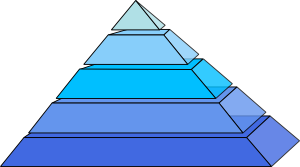
\includegraphics[width=1.1cm]{../Strukturfiler/FIGS/BluePyramid} & \begin{minipage}{\obsl}}{\end{minipage}\\ \end{tabular}\vspace{4mm}\newline}


% = Forudsætning = basis
\newenvironment{basis}{\begin{flushleft} \begin{itshape} }{\end{itshape} \end{flushleft}}


% = Opsummering =
\newenvironment{summary}{\clearpage\pagecolor{sumgul}\section{Opsummering}}{\newpage\pagecolor{white}}











% = Counter
\newcounter{opgavecount}[section]
\setcounter{opgavecount}{0}
\newcounter{spgcount}[opgavecount]
\setcounter{spgcount}{0}
\renewcommand{\thespgcount}{\alph{spgcount})}



% = EXERCISE = (DIVIDER)

\newcommand{\exercisebegin}[1][]{\bigskip\needspace{3\baselineskip}\refstepcounter{opgavecount}\titlegraphic{mingroen}\textcolor{mingroen}{\th{Opgave \theopgavecount \hspace*{1cm} #1}}\medskip\par}

% = QUIZEXERCISE = (DIVIDER)

\newcommand{\quizexercisebegin}[1][]{\bigskip\needspace{3\baselineskip}\refstepcounter{opgavecount}\titlegraphic{mingroen}\textcolor{mingroen}{\th{Quiz-Opgave \theopgavecount \hspace*{1cm} #1}}\medskip\par}

% = QUESTION =

\newenvironment{question}{\refstepcounter{spgcount}\begin{itemize}\item[\thespgcount]}{\end{itemize}\hspace*{\fill}}

% = VINK =

\newenvironment{vink}{\begin{tabular}{m{.9cm}<{\hspace*{2mm}}@{}|m{\obsl}@{}}\hspace*{-4pt}\raggedleft
\includegraphics[width=.9cm]{../Strukturfiler/FIGS/Think} & \begin{minipage}{\obsl}}{\end{minipage}\\ \end{tabular}\medskip\\}
	
% = FACIT =

\newenvironment{facit}{\begin{tabular}{m{.9cm}<{\hspace*{2mm}}@{}|m{\obsl}@{}}\hspace*{-4pt}\raggedleft
\includegraphics[width=.9cm]{../Strukturfiler/FIGS/Check} & \begin{minipage}{\obsl}}{\end{minipage}\\ \end{tabular}\medskip\\}








\newcommand{\afsnit}[1]{\bigskip\th{\titlegraphic{mingroen}\textcolor{mingroen}{#1}} \\ \rule[7pt]{.4\textwidth}{1pt} \vspace*{-2.5mm}\par}

% (DIVIDER):
\newcommand{\ugedagdatotitel}[4]{\pagebreak[4]\section{Semesteruge #1 -- #2 Dag \hspace*{1mm} (#3)} \vspace*{-4mm} \rule[5pt]{\textwidth}{1pt}\vspace*{-2.5mm} \begin{center}\large{\th{#4}}\end{center} \fancyhead[C]{\th{Semesteruge #1}}}

\newenvironment{skema}[1]{\definecolor{shadecolor}{rgb}{0.96,.98, 1.0} \setlength{\FrameSep}{6pt} \renewcommand{\FrameHeightAdjust}{10pt} \vspace*{-4pt}\begin{shaded} \begin{tabular}{#1}}{\end{tabular} \end{shaded} \vspace*{-7pt}}


% ========================

% MAKROER

%\newenvironment{matr}[1][]{\hspace*{-.8mm}\left[\hspace*{-1mm}\begin{array}{#1}}{\end{array}\hspace*{-1mm}\right]\hspace*{-.8mm}}
\newcommand{\bevisslut}{\begin{scriptsize} \begin{flushright} $ \blacksquare $ \end{flushright} \end{scriptsize}}

\newcommand{\tref}[2]{\hyperref[#1]{#2 \ref*{#1}}}
\newcommand{\thref}[2]{\hyperref[#1]{#2}}

\newcommand{\refA}[1]{\colorbox{yellow}{\ref{#1}}}
\newcommand{\hrefA}[2]{\colorbox{yellow}{\href{#1}{#2}}}
\newcommand{\trefA}[2]{\colorbox{yellow}{\hyperref[#1]{#2 \ref*{#1}}}}
\newcommand{\threfA}[2]{\colorbox{yellow}{\hyperref[#1]{#2}}}

\newenvironment{matr}[1]{\hspace*{-.8mm}\begin{bmatrix}\hspace*{-1mm}\begin{array}{#1}}{\end{array}\hspace*{-1mm}\end{bmatrix}\hspace*{-.8mm}}
\newcommand{\transp}{\hspace*{-.6mm}^{\top}}

\newcommand{\maengde}[2]{\left\lbrace \hspace*{-1mm} \begin{array}{c|c} #1 & #2 \end{array} \hspace*{-1mm} \right\rbrace}

\newenvironment{eqnalign}[1]{\setlength{\arraycolsep}{1.3pt}\begin{equation}\begin{array}{#1}}{\end{array}\end{equation}\par}
\newcommand{\eqnl}{\setlength{\arraycolsep}{1.3pt}}

\newcommand{\matind}[3]{{_\mathrm{#1}\mathbf{#2}_\mathrm{#3}}}
\newcommand{\vekind}[2]{{_\mathrm{#1}\mathbf{#2}}}
\newcommand{\jac}[2]{{\mathrm{Jacobi}_\mathbf{#1} (#2)}}
\newcommand{\diver}[2]{{\mathrm{div}\mathbf{#1} (#2)}}
\newcommand{\rot}[1]{{\mathbf{rot}\mathbf{(#1)}}}

\newcommand{\am}{\mathrm{am}}
\newcommand{\gm}{\mathrm{gm}}
\newcommand{\E}{\mathrm{E}}
\newcommand{\Span}{\mathrm{span}}
\newcommand{\mU}{\mathbf{U}}

\newcommand{\ms}{\medskip\\}
\newcommand{\bs}{\bigskip\\}

\newcommand{\mA}{\mathbf{A}}
\newcommand{\mB}{\mathbf{B}}
\newcommand{\mC}{\mathbf{C}}
\newcommand{\mD}{\mathbf{D}}
\newcommand{\mE}{\mathbf{E}}
\newcommand{\mF}{\mathbf{F}}
\newcommand{\mK}{\mathbf{K}}
\newcommand{\mI}{\mathbf{I}}
\newcommand{\mM}{\mathbf{M}}
\newcommand{\mN}{\mathbf{N}}
\newcommand{\mQ}{\mathbf{Q}}
\newcommand{\mT}{\mathbf{T}}
\newcommand{\mV}{\mathbf{V}}
\newcommand{\mW}{\mathbf{W}}
\newcommand{\mX}{\mathbf{X}}
\newcommand{\ma}{\mathbf{a}}
\newcommand{\mb}{\mathbf{b}}
\newcommand{\mc}{\mathbf{c}}
\newcommand{\md}{\mathbf{d}}
\newcommand{\me}{\mathbf{e}}
\newcommand{\mn}{\mathbf{n}}
\newcommand{\mr}{\mathbf{r}}
\newcommand{\mv}{\mathbf{v}}
\newcommand{\mw}{\mathbf{w}}
\newcommand{\mx}{\mathbf{x}}
\newcommand{\mxb}{\mathbf{x_{bet}}}
\newcommand{\my}{\mathbf{y}}
\newcommand{\mz}{\mathbf{z}}
\newcommand{\reel}{\mathbb{R}}
\newcommand{\mL}{\bm{\Lambda}} %Lambda-matrix
\newcommand{\mnul}{\bm{0}}
\newcommand{\trap}[1]{\mathrm{trap}(#1)}
\newcommand{\Det}{\operatorname{Det}}
\newcommand{\adj}{\operatorname{adj}}
\newcommand{\Ar}{\operatorname{Areal}}
\newcommand{\Vol}{\operatorname{Vol}}
\newcommand{\Rum}{\operatorname{Rum}}
\newcommand{\diag}{\operatorname{\bf{diag}}}
\newcommand{\bidiag}{\operatorname{\bf{bidiag}}}
\newcommand{\spanVec}[1]{\mathrm{span}\{#1\}}
\newcommand{\Div}{\operatorname{Div}}
\newcommand{\Rot}{\operatorname{\mathbf{Rot}}}

\newcommand{\Jac}{\operatorname{Jacobi}}
\newcommand{\Tan}{\operatorname{Tan}}
\newcommand{\Ort}{\operatorname{Ort}}
\newcommand{\Flux}{\operatorname{Flux}}
\newcommand{\Cmass}{\operatorname{Cm}}
\newcommand{\Imom}{\operatorname{Im}}
\newcommand{\Pmom}{\operatorname{Pm}}
\newcommand{\IS}{\operatorname{I}}
\newcommand{\IIS}{\operatorname{II}}
\newcommand{\IIIS}{\operatorname{III}}
\newcommand{\Le}{\operatorname{L}}
\newcommand{\app}{\operatorname{app}}
\newcommand{\M}{\operatorname{M}}
\newcommand{\re}{\mathrm{Re}}
\newcommand{\im}{\mathrm{Im}}

\newcommand{\compl}{\mathbb{C}} %de komplekse tal
\newcommand{\e}{\mathrm{e}} %eksponentialfunktionen. lodret 'e', og altså ikke kursiv ligesom andre bogstaver.





% Medialink: SCREEN: (QRcode) + thumbnail image + link på kodenummer (til qr.dtu.dk)
\newcommand{\onlinemedia}[3]{
	\begin{wrapfigure}{r}{3.2cm} 
		\vspace{-30pt} 
		\vspace{#1pt} 
		\begin{flushright} 
			\includegraphics[width=3cm]{qr/#2.png} 
			\tiny 
			\href{http://qr.dtu.dk/#2}{#2: #3}
			\normalsize  
		\end{flushright} 
		\vspace{-10pt} 
	\end{wrapfigure}
}
\newcommand{\onlinemediathumb}[3]{
	\begin{wrapfigure}{r}{3.2cm} 
		\vspace{-30pt} 
		\vspace{#1pt} 
		\begin{flushright} 
			\includegraphics[width=3cm]{qr/#2.png} 
			\includegraphics[width=3cm]{qr/#2_thumb.png} 
			\tiny 
			\href{http://qr.dtu.dk/#2}{#2: #3}
			\normalsize  
		\end{flushright} 
		\vspace{-10pt} 
	\end{wrapfigure}
}



% Index:
\usepackage{makeidx}
\makeindex
\newcommand\ind[2]{\index{#1}\textbf{\textit{\textcolor{black}{#2}}}}

% ###SERVER_EXCLUDE_BEGIN###
\externaldocument[NUID17-]{../../enoten/TN01-Talrum/Talrum}
\externaldocument[NUID1-]{../../enoten/TN02-Ligningssystemer/TNdriver}
\externaldocument[NUID2-]{../../enoten/TN03-Matricer_og_Matrixalgebra/Matricer_og_matrixalgebra}
\externaldocument[NUID3-]{../../enoten/TN04-Kvadratiske_matricer/TNdriver}
\externaldocument[NUID11-]{../../enoten/TN05-Determinanter/Determinanter}
\externaldocument[NUID12-]{../../enoten/TN06-GeometriskeVektorer/GeometriskeVektorer}
\externaldocument[NUID18-]{../../enoten/TN07-Vektorrum/VektorRum}
\externaldocument[NUID21-]{../../enoten/TN08-LinAfbildninger/LinAfbildninger}
\externaldocument[NUID23-]{../../enoten/TN09-Egenvaerdier_og_egenvektorer/TNdriver}
\externaldocument[NUID24-]{../../enoten/TN10-Diagonalisering_med_egenvektorer/TNdriver}
\externaldocument[NUID10-]{../../enoten/TN11-1.ordens_differentialligninger/TNdriver}
\externaldocument[NUID13-]{../../enoten/TN12-1.ordens_differentialligningssystemer/TNdriver}
\externaldocument[NUID14-]{../../enoten/TN13-2.ordens_differentialligninger/TNdriver}
\externaldocument[NUID27-]{../../enoten/TN14-Elemenataere_funktioner/Elementaere_Funktioner}
\externaldocument[NUID28-]{../../enoten/TN15-Funktioner2Variable/Funktioner_To_Variable}
\externaldocument[NUID29-]{../../enoten/TN16-Gradienter_og_Tangentplaner/Gradienter_og_Tangentplaner}
\externaldocument[NUID32-]{../../enoten/TN17-Taylor_formler/Taylor_Formler}
\externaldocument[NUID33-]{../../enoten/TN18-Taylor_2Var/Taylor_2Var}
\externaldocument[NUID34-]{../../enoten/TN19-SymMat/SymmetriskeMatricer}
\externaldocument[NUID35-]{../../enoten/TN20-KegleSnit/Keglesnit}
\externaldocument[NUID36-]{../../enoten/TN21-Riemann_Integral/Riemann_01}
\externaldocument[NUID37-]{../../enoten/TN22-Plan_Int/Plan_Int_01}
\externaldocument[NUID39-]{../../enoten/TN23-Flade_Int/Flade_Rum_Int_01}
\externaldocument[NUID40-]{../../enoten/TN24-Vektorfelter/Vektorfelter_01}
\externaldocument[NUID41-]{../../enoten/TN25-Flux/Flux_02}
\externaldocument[NUID42-]{../../enoten/TN26-Gauss/Gauss_01}
\externaldocument[NUID128-]{../../enoten/TN27-Stokes/Stokes_01}
\externaldocument[NUID43-]{../../enoten/TN29-KomplekseTal/KomplekseTal}

\externaldocument[NUID6-]{../../E-math-opgaver/Opgaver/opgU123}
\externaldocument[NUID19-]{../../E-math-opgaver/Opgaver/opgU45}
\externaldocument[NUID20-]{../../E-math-opgaver/Opgaver/opgU678}
\externaldocument[NUID25-]{../../E-math-opgaver/Opgaver/opgU910SD}
\externaldocument[NUID31-]{../../E-math-opgaver/OpgaverF11-U123/opgF123}
% \externaldocument[NUID9-]{../../E-math-opgaver/Opgaver/Dagsordner E10}
% ###SERVER_EXCLUDE_END###


% Begin document and set alternative chapter title:
\begin{document}
\renewcommand{\chaptername}{eNote}

\setcounter{chapter}{1} %SÆT DETTE TAL TIL 1 MINDRE END DET AKTUELLE ENOTE-NUMMER!!

%%%%%%%%%%%%%%%%%%%%%%%%%%%%%%%%%%%%%%%%%%%%%
%%%%%%%%%%%%%%%%%%%%%%%%%%%%%%%%%%%%%%%%%%%%%
%%% HERFRA SKAL DU SKRIVE ELLER INDSÆTTE %%%%
%%% DEN FIL DU ØNSKER %%%%%%%%%%%%%%%%%%%%%%%
%%%%%%%%%%%%%%%%%%%%%%%%%%%%%%%%%%%%%%%%%%%%%
%%%%%%%%%%%%%%%%%%%%%%%%%%%%%%%%%%%%%%%%%%%%%

\chapter{Lineære ligningssystemer} \label{tn2}

\begin{basis}
Denne eNote handler om lineære ligningssystemer, om metoder til at beskrive dem og løse dem, og om hvordan man kan få overblik over løsningsmængdernes struktur. Noten kan læses uden særlige forudsætninger, dog bør man kende til talrummet $\mathbb R^n$, se \tref{NUID17-tn1}{eNote}.
\end{basis}

\section{Lineære ligninger}

En \ind{lineær ligning}{lineær ligning} med $n$ ubekendte $x_1,\,x_2,\,\ldots\,x_n$ er en ligning af formen
\begin{equation}\label{TN2.1}
a_1\cdot x_1+a_2\cdot x_2+\ldots+a_n\cdot x_n=b\,.
\end{equation}
Tallene $a_1,\,a_2,\,\ldots\,,a_n$ kaldes \textit{koefficienterne} og tallet $b$ kaldes \textit{højresiden}. Koefficienterne og højresiden betragtes som kendte tal i modsætning til de ubekendte. Ligningen kaldes \textit{homogen}, hvis $b=0$, ellers \textit{inhomogen}.

\begin{definition}[Løsning til en lineær ligning]
Ved en \textit{løsning} til ligningen 
\begin{equation}\label{TN2.1b}
a_1\cdot x_1+a_2\cdot x_2+\ldots+a_n\cdot x_n=b\,.
\end{equation}
forstås et talsæt $\mathbf{x}=(x_1,\,x_2,\,\ldots\,,x_n) \in \mathbb R^n$ der ved indsættelse i ligningen får den til at passe, det vil sige at venstresiden er lig med højresiden. \bs
Ved \ind{fuldstændig løsning}{den fuldstændige løsning} eller blot \ind{løsningsmængde}{løsningsmængden} forstås mængden af alle løsninger til ligningen.
\end{definition}


\begin{example}[Ligning for en ret linje i planen]
Et eksempel på en lineær ligning er ligningen for en ret linje i $(x,y)$-planen: 
\begin{equation}\label{TN2.0}
y = 2\, x + 5\,. 
\end{equation}
Her fremstår $y$ isoleret på venstresiden, og koefficenterne 2 og 5 har velkendte geometriske fortolkninger. Men ligningen kunne også skrives som
\begin{equation}
-2\, x_1 + 1\,x_2 = 5
\end{equation}
hvor $x$ og $y$ er erstattet af de mere generelle navne for ubekendte $x_1$ og $x_2$, og hvor ligningen er opskrevet på formen \eqref{TN2.1}.\bs
Løsningsmængden for ligning \eqref{TN2.0} er selvfølgelig koordinatsættene for samtlige punkter på linjen - ved indsættelse vil de jo opfylde ligningen, mens ingen andre gør det!
\end{example}


\begin{example}[Trivielle og inkonsistente ligninger]
Den lineære ligning
\begin{equation}
0x_1+0x_2+0x_3+0x_4=0\,\,\Leftrightarrow\,\,0=0
\end{equation}
hvor alle koefficienterne samt højresiden er $0$, er et eksempel på en \ind{triviel ligning}{triviel} ligning. Ligningens løsningsmængde består af alle $\mathbf x=(x_1,\,x_2,\,x_3,\,x_4) \in \mathbb R^4$.\bs
Hvis alle ligningens koefficienter er $0$, men højresiden er forskellig fra $0$, opstår en \ind{inkonsistent ligning}{inkonsistent} ligning, det vil sige en ligning som ingen løsninger har. Det gælder fx ligningen
\begin{equation}
0x_1+0x_2+0x_3+0x_4=1\,\,\Leftrightarrow\,\,0=1\,.
\end{equation}
\end{example}

Når man undersøger lineære ligninger, kan man benytte de sædvanlige \ind{omformningsregler for ligninger}{om\-form\-nings\-reg\-ler} for ligninger: Man ændrer ikke ved løsningsmængden for ligningen, hvis man lægger den samme størrelse til på begge sider af lighedstegnet, og man ændrer heller ikke ved løsningsmængden hvis man ganger på begge sider af lighedstegnet med en konstant som er forskellig fra $0$.\bs
Alle lineære ligninger som ikke er inkonsistente, og som indeholder mere end én ubekendt, har uendeligt mange løsninger. Det følgende eksempel viser hvordan man i så fald kan opskrive løsnings\-mæng\-den.

\begin{example}[Uendeligt mange løsninger på standard-parameterform]
Vi opstiller en inhomogen lineær ligning med tre ubekendte:  
\begin{equation}\label{TN2.2}
2\,x_1-x_2+4\, x_3=5\,.
\end{equation}
Ved indsættelse af $x_1=1$, $x_2=1$ og $x_3=1$  i ligning (\ref{TN2.2}) ses at $\mathbf x=(1,1,1)$ er en løsning. Men hermed har vi ikke fundet den fuldstændige løsning, da vi for eksempel kan konstatere at $\mathbf x=(\frac 1 2,0,1)$ også er en løsning. Hvordan kan vi angive hele løsningsmængden?\bs
Lad os starte med at isolere $x_1$:
\begin{equation}
x_1=\textstyle \frac 5 2+\frac 1 2\, x_2-2\, x_3\,.
\end{equation}
Til ethvert valg af en talværdi for $x_2$ og en talværdi $x_3$ svarer der netop én ny værdi af $x_1$. Lad os fx sætte $x_2=1$ og $x_3=4$, så får vi $x_1=-5$. Det betyder at talsættet $(-5,1,4)$ er en løsning. Vi kan derfor betragte $x_2$ og $x_3$ som \textit{frie parametre}, der fastlægger værdien af $x_1$. Vi \textbf{omdøber} derfor $x_2$ og $x_3$ til parameter-navnene $s$ henholdsvis $t$ således: $s=x_2$ og $t=x_3$. Hvorefter $x_1$ kan udtrykkes således:
\begin{equation}
x_1=\textstyle \frac 5 2+\frac 1 2\, x_2-2\, x_3
   =\textstyle \frac 5 2+\frac 1 2\, s-2\,t\,.
\end{equation}
Vi kan nu opskrive den fuldstændige løsning for ligning (\ref{TN2.2}) på følgende \ind{standard-parameterform}{standard-parameterform}:
\begin{equation}\label{TN2.3}
\mathbf x =
\begin{matr}{r} x_1\\ x_2\\ x_3 \end{matr} =
\begin{matr}{r} \frac 5 2\\ 0\\ 0\end{matr}+s\cdot \begin{matr}{r} \frac 1 2\\ 1\\ 0\end{matr}+t\cdot \begin{matr}{r} -2\\ 0\\ 1\end{matr} \,\, \mathrm{hvor} \,\,s,t\in\mathbb{R}\,.
\end{equation}

Bemærk at parameterfremstillingens midterste ligning $\,x_2=0+s\cdot 1 + t\cdot 0\,$ sådan set blot udtrykker navneskiftet $x_2\rightarrow s$. Tilsvarende udtrykker den nederste blot navneskiftet $x_3\rightarrow t$.
\end{example}

\begin{aha}
Hvis vi opfatter ligning (\ref{TN2.2}) som ligningen for en plan i rummet, så angiver ligning (\ref{TN2.3}) en \textit{parameterfremstilling} for den samme plan. Første søjlevektor på højresiden angiver \textit{begyndelsespunktet} i planen, og de to sidste søjlevektorer er \textit{retningsvektorer} for planen. Dette er beskrevet nærmere i \tref{NUID12-tn6}{eNote}, som hedder ``Geometriske vektorer''.
\end{aha}

%HER er fjernet en opgave%

%%%%%%%%%%%%%%%%%%%%%%%%%%%%%%%%%%%%%%%%%%%%%%%%%%%%%%%%%%%%%%%%%%%%%%%%%%%%%%%%%
\section{System af lineære ligninger}

Et \ind{lineært ligningssystem}{lineært ligningssystem} bestående af $m$ lineære ligninger med $n$ ubekendte skrives på formen
\begin{eqnalign}{rcrcrcrcl}\label{linLignSystem} 
a_{11}\cdot x_1 &+& a_{12}\cdot x_2 &+& \ldots &+& a_{1n}\cdot x_n &=& b_1\\
a_{21}\cdot x_1 &+& a_{22}\cdot x_2 &+& \ldots &+& a_{2n}\cdot x_n &=& b_2\\
 &&  &\vdots & && &&\\
a_{m1}\cdot x_1 &+& a_{m2}\cdot x_2 &+& \ldots &+& a_{mn}\cdot x_n &=& b_m
\end{eqnalign}
Ligningssystemet har $m$ \textit{rækker}, som hver indeholder en ligning. De $n$ ubekendte, som betegnes $x_1,\,x_2,\,\ldots\,x_n\,$, optræder i hver af de $m$ ligninger, hvis ikke kan vælger at udelade eventuelle led, hvis koefficient er $0$. Koefficienten til $x_j$ i ligningens række nummer $i$ betegnes $a_{ij}$. Ligningssystemet kaldes \textit{homogent}, hvis alle de $m$ højresiders $b_i$ er lig med $0$, i modsat fald  \textit{inhomogent}.

\begin{definition}[Løsning til et lineært ligningssystem]
Ved en \textit{løsning} til det lineære ligningssystem
\begin{eqnalign}{rcrcrcrcl} \label{TN2.4b}
a_{11}\cdot x_1 &+& a_{12}\cdot x_2 &+& \ldots &+& a_{1n}\cdot x_n &=& b_1\\
a_{21}\cdot x_1 &+& a_{22}\cdot x_2 &+& \ldots &+& a_{2n}\cdot x_n &=& b_2\\
 &&  &\vdots & && &&\\
a_{m1}\cdot x_1 &+& a_{m2}\cdot x_2 &+& \ldots &+& a_{mn}\cdot x_n &=& b_m
\end{eqnalign}
forstås et talsæt $\mathbf{x}=(x_1,\,x_2,\,\ldots\,x_n) \in \mathbb R^n$ der ved indsættelse får alle de $m$ lineære ligninger i systemet til at passe, det vil sige at venstresiden i hver ligning er lig med højresiden.\bs
Ved \ind{fuldstændig løsning}{den fuldstændige løsning} eller blot \ind{løsningsmængde}{løsningsmængden} forstås mængden af alle løsninger til ligningssystemet. En enkelt løsning betegnes ofte som en \ind{partikulær løsning}{partikulær} løsning. 
\end{definition}

\begin{example}[Homogent lineært ligningssystem]
Der er givet et homogent lineært ligningssystem af to ligninger med fire ubekendte:
\begin{eqnalign}{rcrcrcrcl} \label{TN2.5}
x_1 &+& x_2 &+& 2\,x_3 &+& x_4 &=& 0 \\
2\,x_1 &-& x_2 &-& x_3 &+& x_4 &=& 0
\end{eqnalign}
Vi vil undersøge om talsættene $\mathbf{x}=(1,1,2,-6)$ og $\mathbf{y}=(3,0,1,-5)$ er partikulære løsninger til ligningerne (\ref{TN2.5}). Ved indsættelse af $\mathbf{x}$ i systemets venstreside får vi
\begin{equation}
\begin{array}{r}
1+1+2\cdot 2-6=0\\
2\cdot 1-1-2-6=-7
%\end{array}
%\hspace{0.5cm}\Leftrightarrow \hspace{0.5cm}
%\begin{array}{r}
%0=0\\
%-7=0
\end{array}
\end{equation}
Da venstresiden kun i det første tilfælde er lig med den givne højreside $0\,$, er $\mathbf{x}$ kun en løsning til den første af de to ligninger. Derfor er $\mathbf{x}$ ikke en løsning til ligningssystemet.\bs
Ved indsættelse af $\mathbf{y}$ får vi
\begin{equation}
\begin{array}{r}
3+0+2\cdot 1-5=0\\
2\cdot 3-0-1-5=0
%\end{array}
%\hspace{0.5cm}\Leftrightarrow \hspace{0.5cm}
%\begin{array}{r}
%0=0\\
%0=0
\end{array}
\end{equation}
Da venstresiden i begge tilfælde er lig med den givne højreside $0\,$, er $\mathbf{y}$ løsning til begge de to ligninger. Derfor er $\mathbf{y}$ en partikulær løsning til ligningssystemet.
\end{example}

\begin{aha}
Løsningsmængden til et lineært ligningssystem er \ind{fællesmængde}{fællesmængden} af løsningsmængderne til hver af de ligninger som indgår i systemet.
\end{aha}

%%%%%%%%%%%%%%%%%%%%%%%%%%%%%%%%%%%%%%%%%%%%%%%%%%%%%%%%%%%%%%%%%%%%%%%%%%%%%%%%%%%%%%%%%
\section{Koefficientmatrix og totalmatrix}

Når man skal undersøge et lineært ligningssystem er det ofte bekvemt at benytte sig af \textit{matricer}. En \ind{matrix}{matrix} er et rektangulært talskema som består af et vist antal rækker og søjler. For eksempel har matricen $\mathbf M$, givet ved
\begin{equation}
\mathbf M=\begin{matr}{rrr} 1&0&5 \\ 8&3&2 \end{matr} \,,
\end{equation}
to rækker og tre søjler. De seks tal kaldes matricens \ind{element i matrix}{elementer}. Matricens \ind{diagonal i matrix}{diagonal} består af de elementer, hvis rækkenummer er lig med søjlenummer. I $\mathbf M$ består diagonalen således af elementerne 1 og 3.\bs
Ved \textit{koefficientmatricen} $\mathbf A$ til det lineære ligningssystem (\ref{linLignSystem}) forstås den matrix hvis første række består af koefficienterne til den første ligning, hvis anden række består af koefficienterne til den anden ligning og så videre. Kort sagt den følgende matrix med $m$ rækker og $n$ søjler:
\begin{equation}
\mathbf{A}=
\begin{matr}{cccc}
 a_{11} & a_{12} & \cdots & a_{1n} \\
 a_{21} & a_{22} & \cdots & a_{2n} \\
 \vdots&\vdots&&\vdots\\
 a_{m1}&a_{m2}&\cdots&a_{mn}
\end{matr}
\end{equation}
Ligningssystemets \textit{totalmatrix} $\mathbf T$ fremkommer ved at man i koeffecientmatricens højre side tilføjer en ny søjle som består af ligningssystemets højresider $b_i$. $\mathbf T$ har dermed $m$ rækker og $n+1$ søjler. Hvis vi samler højresiderne $b_i$ i en søjlevektor $\mathbf b$, som vi kalder \textit{ligningssystemets højreside}, er $\mathbf T$ sammensat således hvor den lodrette hjælpelinje symboliserer systemets lighedstegn:
\begin{equation}\label{totalMatrixMedLodretLinje}
\mathbf T= \begin{matr}{c|c} \mathbf A & \mathbf b \end{matr}
=
\begin{matr}{cccc|c}
 a_{11} & a_{12} & \cdots & a_{1n} & b_1\\
 a_{21} & a_{22} & \cdots & a_{2n} & b_2\\
 \vdots&\vdots&&\vdots&\vdots\\
 a_{m1}&a_{m2}&\cdots&a_{mn} & b_m
\end{matr}
\end{equation}

\begin{aha}
Den lodrette hjælpelinje før sidste søjle i (\ref{totalMatrixMedLodretLinje}) har blot den pædagogiske funktion at skabe klarere overblik. Man kan vælge at udelade linjen hvis det i sammenhængen ikke kan føre til misforståelser.
\end{aha}

\begin{example}[Koefficientmatrix, højresider og totalmatrix]
For det følgende lineære ligningssystem af 3 ligninger med 3 ubekendte
\begin{eqnalign}{rcrcrcl}
&& -x_2 &+& x_3 &=& 2\\
2x_1 &+& 4x_2 &-& 2x_3 &=& 2\\
3x_1 &+& 4x_2 &+& x_3 &=& 9
\end{eqnalign}
har vi 
\begin{equation}
\mathbf{A}=
\begin{matr}{rrr}
 0&-1& 1 \\
 2& 4&-2 \\
 3& 4& 1
\end{matr} \; , \quad
\mathbf{b} =
\begin{matr}{r}
 2\\2\\9
\end{matr} \quad \mathrm{og} \quad
\mathbf{T}=
\begin{matr}{rrr|r}
 0&-1& 1 & 2\\
 2& 4&-2 & 2\\
 3& 4& 1 & 9
\end{matr}
\end{equation}
Bemærk at det $0$ som er placeret øverst til venstre i $\mathbf{A}$ og $\mathbf{T}$, angiver at koefficienten til $x_1$ i ligningssystemets øverste række er $0$.
\end{example}

\begin{aha}
Det smarte ved en koefficientmatrix (og en totalmatrix) er at vi ikke behøver at skrive de ubekendte op. Koefficienternes entydige placering i matricen gør at vi ikke er i tvivl om hvilken af de ubekendte hver af dem hører til. Vi har fjernet overflødige symboler!
\end{aha}

%%%%%%%%%%%%%%%%%%%%%%%%%%%%%%%%%%%%%%%%%%%%%%%%%%%%%%%%%%%%%%%%%%%%%%%%%%%
\section{Reduktion af lineære ligningssystemer}
Lineære ligningssystemer kan reduceres, det vil sige gøres enklere, ved hjælp af en metode der kaldes Gauss-elimination. Metoden har flere forskellige varianter, og den særlige variant der benyttes i disse eNoter, går under navnet \ind{GaussJordan-elimination}{GaussJordan-elimination}. Det algebraiske grundlag for alle varianterne er at man kan omforme et lineært ligningssy\-stem ved såkaldte \ind{rækkeoperationer}{rækkeoperationer} uden at man derved ændrer på ligningssystemets løsningsmængde. Når ligningssystemet er reduceret mest muligt, er det som regel nemt at aflæse og opskrive dets løsningsmængde.

\begin{theorem}[Rækkeoperationer]\label{TN2.6}
Man ændrer ikke på et lineært ligningssystems løsnings\-mængde hvis man omformer ligningssystemet ved en af de følgende tre \ind{rækkeoperationer}{rækkeoperationer}:
\begin{enumerate}
\item[ro$_1$:] Lader to af ligningerne bytte række.
\item[ro$_2$:] Ganger en af ligningerne med en konstant som ikke er $0$.
\item[ro$_3$:] Til en ligning lægger en af de øvrige ligninger ganget med en konstant.
\end{enumerate}
\end{theorem}

\begin{info}%[Notation for rækkeoperationer]
Vi fastlægger her en kort notation for hver af de tre rækkeoperationer: \medskip \\
\begin{tabular}{lrl}
ro$_1$:& $R_i\leftrightarrow R_j\,$:& Ligningen i række $i$ ombyttes med ligningen i række $j$.\medskip \\ 
ro$_2$:&$k\cdot R_i\,$:& Ligningen i række $i$ ganges med $k$.\medskip \\ 
ro$_3$:&$R_j+k\cdot R_i\,$:& Til ligningen i række $j$ lægges ligningen i række $i$ ganget med $k$.
\end{tabular}
\end{info}

I det følgende eksempel afprøver vi de tre rækkeoperationer.

\begin{example}[Rækkeoperationerne]
Vi eksemplificerer ro$_1$: Betragt ligningssystemet nedenfor til venstre. Vi ombytter de to ligninger i de to rækker, hvorved vi har udført $R_1\leftrightarrow R_2\,$.
\begin{equation}
\eqnl
\begin{array}{rcrcl}
x_1 &+& 2x_2 &=& -3\\
x_1 &+& x_2 &=& 0
\end{array}
\quad \rightarrow \quad
\begin{array}{rcrcl}
x_1 &+& x_2 &=& 0\\
x_1 &+& 2x_2 &=& -3
\end{array}
\end{equation}
Systemet til højre har samme løsningsmængde som systemet til venstre.\bs
Vi eksemplificerer ro$_2$: Betragt ligningssystemet nedenfor til venstre. Vi ganger ligningen i den anden række med $5$, hvorved vi har udført $5\cdot R_2\,$:
\begin{equation}
\eqnl
\begin{array}{rcrcl}
x_1 &+& 2x_2 &=& -3\\
x_1 &+& x_2 &=& 0
\end{array}
\quad \rightarrow \quad
\begin{array}{rcrcl}
x_1 &+& 2x_2 &=& -3\\
5\,x_1 &+& 5\,x_2 &=& 0
\end{array}
\end{equation}
Systemet til højre har samme løsningsmængde som systemet til venstre.\bs
Vi eksemplificerer ro$_3$: Betragt ligningssystemet nedenfor til venstre. Til ligningen i dets nederste række lægger vi ligningen i den øverste række ganget med $2$. Vi har dermed udført $R_2+2\cdot R_1\,$:
\begin{equation}
\eqnl
\begin{array}{rcrcl}
x_1 &+& 2x_2 &=& -3\\
x_1 &+& x_2 &=& 0
\end{array}
\quad \rightarrow \quad
\begin{array}{rcrcl}
x_1 &+& 2x_2 &=& -3\\
3x_1 &+& 5x_2 &=& -6
\end{array}
\end{equation}
Systemet til højre har samme løsningsmængde som systemet til venstre.

\begin{aha}
Pilen, $ \rightarrow $, som er brugt i de tre eksempler, indikerer at en (eller flere) rækkeoperation(er) har fundet sted.
\end{aha}
\end{example}

\begin{bevis}%[for sætning \ref{TN2.6}]
Første del af beviset for sætning \ref{TN2.6} er enkelt: Da løsningsmængden for et ligningssystem er identisk med \emph{fællesmængden} $F$ af løsningsmængderne til hver af de ligninger der indgår i systemet, ændres $F$ naturligvis ikke ved at ligningernes rækkefølge ændres. Derfor er ro$_1$ tilladt.\bs
%At de to sidste rækkeoperationer heller ikke ændrer ligningssystemets løsningsmængde kan forklares ud fra sædvanlige \textit{omformningsregler} for én ligning på følgende måde:\bs
Da én lignings løsningsmængde ikke ændres ved at den ganges med en konstant $k\neq 0$, vil $F$ ikke kunne påvirkes af at en af ligningerne i et ligningssystem erstattes af ligningen selv ganget med en konstant forskellig fra $0$. Derfor er ro$_2$ tilladt.\bs
Betragt endelig et lineært ligningssystem $A$ med $n$ ubekendte $\mx=(x_1,\,x_2,\,\ldots\,x_n)$. Venstresiden af en ligning i $A$ opskriver vi som $\,L(\mx)\,$ og højresiden som $b\,$. Vi udfører nu en vilkårlig rækkeoperation af typen ro$3$ på følgende måde: En vilkårlig ligning $\,L_1(\mx)=b_1\,$ ganges med et vilkårligt reelt tal $k$ og lægges dernæst til en vilkårlig anden ligning $\,L_2(\mx)=b_2\,$. Herved dannes en ny ligning $\,L_3(\mx)=b_3\,$ hvor
$$L_3(\mx)=L_2(\mx)+k\,L_1(\mx)\,\,\,\mathrm{og}\,\,\,b_3=b_2+k\,b_1\,.
$$
Vi viser nu at det ligningssystem $B$, som opstår ved at $\,L_2(\mx)=b_2\,$ i $A$ erstattes af $\,L_3(\mx)=b_3\,$, har samme løsningsmængde som $A$, og at ro$_3$ dermed er tilladt. Antag først at $\mx_0$ er en vilkårlig løsning til $A\,$. Så gælder i følge omformningsregler for én ligning at 
$$k\,L_1(\mx_0)=k\,b_1$$
og videre at  
$$L_2(\mx_0)+k\,L_1(\mx_0)=b_2+k\,b_1\,.$$
Heraf følger at $\,L_3(\mx_0)=b_3\,$, og dermed at $\mx_0$ også er en løsning til $B$. Antag nu omvendt at $\mx_1$ er en vilkårlig løsning til $B\,$. Så følger på samme måde at $$-k\,L_1(\mx_1)=-k\,b_1\,$$ og videre at $$L_3(\mx_1)-k\,L_1(\mx_1)=b_3-k\,b_1\,.$$
Det betyder at $\,L_2(\mx_1)=b_2\,$, og at $\mx_1$ også er en løsning til $A$. Samlet er det som ønsket vist at ro$_3$ er tilladt.

%Lad os til sidst kalde de to ligninger ro$_3$ handler om, for henholdsvis $a_1$ og $b$. Vi ganger $a_1$ med en konstant $k$ og opnår herved en ny ligning $a_2$. Når vi herefter lægger $a_2$ til $b$, opnår vi igen en ny ligning $c$. Vi skal vise at løsningsmængden $L(a_1,c)$ for ligningssystemet bestående af $a_1$ og $c$ er identisk med løsningsmængden $L(a_1,b)$ for ligningssystemet bestående af $a_1$ og $b$.\\

%Dette er klart hvis $k=0$, da $b$ og $c$ i så fald er identiske. Vi indskrænker os i det følgende til $k\neq 0$.\\

%Antag først at talsættet $\mathbf x$ tilhører $L(a_1,b)$. Så er $\mathbf x$ en løsning til både $a_1$ og $b$. $\mathbf x$ er også en løsning til $a_2$, da $a_2$ jo er fremkommet af $a_1$ ved gangning af $a_1$ med en konstant der ikke er $0$. Men så er $\mathbf x$ også en løsning til $c$. For at indse dette indsætter vi $\mathbf x$ i både $a_2$ og $b$. Så er venstresiden af $a_2$ lig med højresiden af $a_2$, og venstresiden af $b$ lig med højresiden af $b$. Og derved er summen af venstresiderne af $a_2$ og $b$ lig med summen af højresiderne af $a_2$ og $b$. Hvilket er det samme som at venstresiden af $c$ er lig med højresiden af $c$ når $\mathbf x$ er indsat i $c$. Altså er $\mathbf x$ en løsning til $c$, og derved er det vist at $\mathbf x$ tilhører $L(a_1,c)$.\\

%Antag herefter omvendt at talsættet $\mathbf x$ tilhører $L(a_1,c)$. Så kan vi med helt tilsvarende argumenter vise at $\mathbf x$ også tilhører $L(a_1,b)$ (vi kommer tilbage ved den modsatte rækkeoperation). Derfor er $L(a_1,c)$ identisk med $L(a_1,b)$. Og derfor må løsningsmængden for hele det givne ligningssystem være den samme som for det ligningssystem der fremkommer når ligning $b$ erstattes af ligning $c\,$. Hermed er det vist at ro$_3$ er tilladt.\\

\end{bevis}

Af  sætning \ref{TN2.6} får vi umiddelbart:

\begin{corollary}
Man ændrer ikke på et lineært ligningssystems løsningsmængde hvis man omformer det et vilkårligt antal gange og i en vilkårlig rækkefølge ved hjælp af de tre rækkeoperationer.
\end{corollary}

Vi er nu rede til at benytte de tre rækkeoperationer til at reducere et lineært lig\-nings\-sy\-stem. Vi følger i det følgende eksempel principperne i \textit{GaussJordan-elimination}, og vil senere i afsnit \ref{TN2.13e} give en præcis karakteristik af denne metode.

\begin{example}[GaussJordan-elimination]\label{TN2.8}
Vi betragter nedenfor til venstre et lineært ligningssystem, som består af tre ligninger hvori der indgår de tre ubekendte $x_1$, $x_2$ og $x_3$. Til højre er ligningssystemets \textit{totalmatrix} opskrevet:
\begin{equation}\label{TN2.8b}
\begin{aligned}
-x_2 + x_3 &= 2\\
2x_1 + 4x_2 - 2x_3 &= 2\\
3x_1 + 4x_2 + x_3 &= 9
\end{aligned}
\quad \quad
\mathbf{T}=
\begin{matr}{rrr|r}
 0&-1& 1 & 2\\
 2& 4&-2 & 2\\
 3& 4& 1 & 9
 \end{matr}
\end{equation}
Ideen i reduktionen er gennem rækkeoperationerne at opnå følgende situation: $x_1$ er det eneste tilbageværende led på venstresiden af den øverste ligning, $x_2$ er det eneste venstresiden af den mellemste ligning, og $x_3$ er det eneste på venstresiden af den nederste ligning. \textit{Hvis} dette er muligt, er ligningssystemet ikke blot reduceret, men også løst! 
Vi går frem efter en række trin, som følger GaussJordan-algoritmen. Samtidig ser vi på rækkeoperationernes indvirk\-ning på totalmatricen.\bs
Først ønsker vi at den ligning som opføres i den øverste række, faktisk indeholder  $x_1$, og at $x_1$ har koefficienten $1$. Det kan vi opnå i to trin. Vi ombytter de to øverste ligninger, og ganger derefter den ligning som nu står i øverste række, med $\frac 1 2$. Kort sagt
\begin{equation}
\begin{gathered}
R_1\leftrightarrow R_2 \quad \mathrm{og}\quad \frac 1 2 \cdot R_1\,: \\
\begin{aligned}
x_1 + 2x_2 - x_3&=1\\
-x_2+x_3&=2 \\
3x_1+4x_2+x_3&=9
\end{aligned}
\quad \quad
\begin{matr}{rrr|r}
 1& 2&-1&1 \\
 0&-1& 1&2 \\
 3& 4& 1&9
\end{matr}
\end{gathered}
\end{equation}
Nu fjerner vi alle andre forekomster af $x_1$. I dette eksempel er der kun én forekomst der skal fjernes, nemlig i række $3$. Det opnås således: Vi ganger  ligningen i række $1$ med tallet $-3$ og lægger dette produkt til ligningen i række $3$, kort sagt
\begin{equation} 
\begin{gathered}
R_3 - 3\cdot R_1: \\
\begin{aligned}
x_1+ 2x_2 - x_3&=1\\
-x_2+x_3&=2 \\
-2x_2+4x_3&=6
\end{aligned}
\quad \quad
\begin{matr}{rrr|r}
 1& 2&-1&1 \\
 0&-1& 1&2 \\
 0&-2& 4&6
\end{matr}
\end{gathered}
\end{equation}
Vi har nu opnået at $x_1$ som ønsket kun optræder i række $1$. Der skal den blive! Arbejdet med $x_1$ er afsluttet. Dette svarer til at der øverst i totalmatricens første søjle er et $1$-tal og under $1$-tallet kun $0$-er. Det vil sige at arbejdet med første søjle er færdiggjort!\bs
De næste omforminger skal undersøge om vi på samme måde kan sikre at den ubekendte $x_2$ kun er repræsenteret i række $2$. Først sørger vi lige for at koefficienten for $x_2$ i række $2$ skifter koefficient fra $-1$ til $1$ med operationen
\begin{equation}
\begin{gathered}
(-1)\cdot R_2\,: \\
\begin{aligned}
x_1+2x_2-2x_3&=1\\
x_2-x_3&=-2 \\
-2x_2+4x_3&=6
\end{aligned}
\quad \quad
\begin{matr}{rrr|r}
 1& 2&-1&1 \\
 0& 1&-1&-2\\
 0&-2& 4&6
\end{matr}
\end{gathered}
\end{equation}
Nu kan vi fjerne forekomsterne af $x_2$ fra række 1 og række 3 med operationerne
\begin{equation}
\begin{gathered}
R_1 - 2\cdot R_2 \quad \mathrm{og} \quad R_3 + 2\cdot R_2: \\
\begin{aligned}
x_1+x_3&=5\\
x_2-x_3&=-2 \\
2x_3&=2
\end{aligned}
\quad \quad
\begin{matr}{rrr|r}
 1& 0& 1&5 \\
 0& 1&-1&-2 \\
 0& 0& 2&2
\end{matr}
\end{gathered}
\end{equation}
Herefter er arbejdet med $x_2$ afsluttet, hvilket svarer til at der i række $2$ i totalmatricens anden søjle er et $1$-tal, og $0$ ovenfor og nedenunder. Denne søjle må ikke ændres ved efterfølgende operationer.\bs
Til sidst ønsker vi at den ubekendte $x_3$ er repræsenteret i række $3$ med koefficienten $1$, og at $x_3$ fjernes fra række $1$ og række $2$. Det kan vi opnå vi i to trin. Først
\begin{equation} 
\begin{gathered}
\frac 1 2 \cdot R_3: \\
\begin{aligned}
x_1+x_3&=5\\
x_2-x_3&=-2\\
x_3&=1
\end{aligned}
\quad \quad
\begin{matr}{rrr|r}
 1& 0& 1&5\\
 0& 1&-1&-2\\
 0& 0& 1&1
\end{matr}
\end{gathered}
\end{equation}
Derefter
\begin{equation} \label{TN2.7}
\begin{gathered}
R_1 - R_3 \quad \mathrm{og}\quad R_2 + R_3: \\
\begin{aligned}
x_1&=4\\
x_2&=-1 \\
x_3&=1
\end{aligned}
\quad \quad
\begin{matr}{rrr|r}
 1& 0& 0&4 \\
 0&  1& 0&-1 \\
 0& 0&  1&1
\end{matr}
\end{gathered}
\end{equation}
Nu optræder $x_3$ kun i række $3$. Det svarer til at der i række $3$ i totalmatricens tredje søjle er et $1$-tal, og $0$-er i de andre rækker i denne søjle. Vi har nu gennemført en \textit{fuldstændig reduktion} af ligningssystemet, og vi kan af dette resultat konkludere at der findes netop én løsning til det ligningssystem vi har arbejdet med, nemlig:
\begin{equation}\label{TN2.8d}
\mathbf{x}=(x_1,x_2,x_3)=(4,-1,1).
\end{equation}
\end{example}

\begin{aha}
Lad os huske hvad en løsning er: Et talsæt der får alle ligningerne i ligningssystemet til at passe! Lad os eftervise at formel (\ref{TN2.8d}) faktisk er en løsning til ligningssystemet i ligning (\ref{TN2.8b}):

$$
\begin{aligned}
-(-1) + 1 &= 2\\
2\cdot 4 + 4\cdot(-1) - 2\cdot 1 &= 2\\
3\cdot 4 + 4\cdot(-1) + 1 &= 9
\end{aligned}
$$
Som forventet passer alle tre ligninger!

\end{aha}

I \eqref{TN2.7} har ligningssystemets totalmatrix efter ræk\-ke\-ope\-ra\-tion\-er\-ne opnået en særlig smuk form med tre såkaldt ledende $1$-taller i \ind{diagonal i matrix}{diagonalen} og $0$-er alle andre steder. Man siger at den omformede matrix er en \textit{trappematrix}, idet de ledende $1$-taller danner en trappe man kan gå nedad fra venstre mod højre! Det er dog ikke altid muligt at få trappens $1$-taller til at følge en ret linje, men mindre kan også gøre det! Ofte må man flytte sig mere end én søjle mod højre for at finde næste trin. Den generelle lidt kringlede definition følger herunder.  

\begin{definition}[Trappematrix]\label{TN2.13}
Et lineært ligningssystem kaldes et \ind{fuldstændigt reduceret ligningssystem}{fuldstændigt reduceret ligningssystem}, hvis dets tilhørende totalmatrix er en \ind{trappematrix}{trappematrix}. En matrix er en trappematrix, hvis den opfylder de følgende fire betingelser:
\begin{enumerate}
\item Det første tal i en række, som ikke er et $0$, skal være et $1$-tal. Det kaldes for rækkens \ind{ledende 1-tal}{ledende $1$-tal}.
\item I to på hinanden følgende rækker, som begge har et ledende $1$-tal, står den øverste rækkes ledende $1$-tal længere til venstre end den følgende rækkes ledende 1-tal (trappen går nedad fra venstre mod højre). 
\item I en søjle hvori der optræder et ledende $1$-tal, består de øvrige elementer i søjlen udelukkende af $0$-er.
\item Eventuelle rækker som udelukkende består af $0$-er, er  placeret i bunden af matricen.
\end{enumerate}
\end{definition}



\begin{info}
Definitionen på en trappematrix fra \tref{TN2.13}{Definition} betegnes i den internationale litteratur som, at matricen har \textit{reduced row echelon form}.
\end{info}

\begin{example}[Trappematricer]
Betragt de følgende tre matricer
\begin{equation}
\mathbf{A}=\begin{matr}{rrr}
 \mathbf 1& 0& 0 \\
 0& \mathbf 1& 0 \\
 0& 0&  \mathbf 1
\end{matr} \;, \quad
\mathbf{B}=\begin{matr}{rrr}
\mathbf 1& 2& 0 \\
 0& 0& \mathbf 1 \\
 0& 0&  0
\end{matr} \quad \mathrm{og} \quad
\mathbf{C}=\begin{matr}{rrr}
 \mathbf 1& 3& 1 \\
 0&  0& 0 \\
 0& 0&  0
\end{matr} \,.
\end{equation}
De tre viste matricer er alle trappematricer. De ledende 1-taller betragtes som trappens ``trin''. I $\mathbf{A}$ er trinene smukt placeret i \textit{diagonalen}. $\mathbf{B}$ har kun to ledende 1-taller, og man må gå to søjler mod højre for at komme fra første til andet trin. I $\mathbf{C}$ har trappen kun ét trin. 
\end{example}

\begin{example}
Ingen af de følgende fire matricer er trappematricer, idet hver af dem strider mod netop én af reglerne i definition \ref{TN2.13}. Det overlades til læseren at afgøre hvilken!
\begin{equation}
\mathbf{A}=\begin{matr}{rrr}
 1& 1& 0 \\
 0& 1& 0 \\
 0& 0& 1
\end{matr} \; , \quad
\mathbf{B}=\begin{matr}{rrr}
 0& 0&  0\\
 1& 2& 0 \\
 0& 0& 1 
\end{matr} \; , \quad
\mathbf{C}=\begin{matr}{rrr}
 1& 0& 0 \\
 0& 2& 1 \\
 0& 0& 0
\end{matr} \quad \mathrm{og} \quad
\mathbf{D}=\begin{matr}{rrr}
 1& 0& 0 \\
 0& 0& 1 \\
 0& 1& 0
\end{matr} \,.
\end{equation}
\end{example}

Der gælder nu følgende vigtige sætning om forholdet mellem en matrix og den trappematrix som den kan omformes til ved hjælp af rækkeoperationer:

\begin{theorem}[Trappeform]\label{TN2.13b}
Hvis en given matrix $\mathbf{M}$ ved to forskellige serier af rækkeoperationer er blevet omformet til en trappematrix, så er de to fremkomne trappematricer identiske.\bs
Den unikke trappematrix som en given matrix $\mathbf{M}\,$ kan omformes til ved hjælp af rækkeoperationer, kaldes matricens \ind{trappeform}{trappeform}, og den har symbolet trap$(\mathbf{M})$.
\end{theorem}

\begin{bevis}
Vi benytter følgende model over de seks matricer som introduceres i løbet af beviset:
\begin{equation}
\begin{array}{llcrr}
\mathbf{A}&\stackrel{f_1}{\longleftarrow}&\mathbf{M}&\stackrel{f_2}{\longrightarrow}&\mathbf{B}\\
&&\downarrow&&\\
\mathbf{A}_1&\stackrel{f_1}{\longleftarrow}&\mathbf{M}_1&\stackrel{f_2}{\longrightarrow}&\mathbf{B}_1
\end{array}
\end{equation}
Antag at en matrix $\mathbf{M}$ ved to forskellige serier af rækkeoperationer $f_1$ og $f_2$ er blevet omformet til to forskellige trappematricer $\mathbf{A}$ og $\mathbf{B}$. Lad søjle nummer $k$ være den første søjle i $\mathbf{A}$ og $\mathbf{B}$ hvor de to matricer afviger fra hinanden. Vi danner nu en ny matrix $\mathbf{M}_1$ ud af $\mathbf{M}$ på følgende måde. Først fjerner vi alle de søjler i $\mathbf{M}$ hvis søjlenummer er større end $k$ . Dernæst fjerner vi netop de søjler i $\mathbf{M}$ hvis søjlenummer er mindre end $k\,$, og som har samme søjlenummer som en søjle i $\mathbf{A}$ (og dermed $\mathbf{B}$) der ikke indeholder et ledende $1$-tal.\bs
Nu omformer vi $\mathbf{M}_1$ ved rækkeoperationsfølgerne $f_1$ og $f_2$, og de matricer der dannes herved kalder vi for $\mathbf{A}_1$ henholdsvis $\mathbf{B}_1$. Da vil $\mathbf{A}_1$ nødvendigvis være den samme matrix, som vil fremkomme hvis vi fra $\mathbf{A}$ fjerner alle de søjler, der svarer til dem vi fjernede fra $\mathbf{M}$ for at opnå $\mathbf{M}_1$. Og det samme forhold er der mellem $\mathbf{B}_1$ og $\mathbf{B}$. $\mathbf{A}_1$ og $\mathbf{B}_1$ vil derfor have ledende $1$-taller i diagonalen i alle søjler på nær den sidste søjle, som er den første søjle hvor de to matricer er forskellige fra hinanden. I denne sidste søjle er der to muligheder: Enten har én af matricerne et ledende $1$-tal i denne søjle eller også har ingen af dem det. Et eksempel på hvordan situationen i det første tilfælde kunne være, er:
\begin{equation}
\mathbf{A}_1=
\begin{matr}{rrr}
 1& 0& 0 \\
 0&  1& 0 \\
 0& 0&  1
\end{matr} \quad \quad
\mathbf{B}_1=
\begin{matr}{rrr}
 1& 0& 0 \\
 0& 1& 2 \\
 0& 0& 0
\end{matr}
\end{equation}
Vi fortolker nu $\mathbf{M}_1$ som totalmatrix for et lineært ligningssystem $\mathcal L\,$. Både $\mathbf{A}_1$ og $\mathbf{B}_1$ vil da repræsentere et fuldstændigt reduceret ligningssystem der skal have samme løs\-nings\-mæng\-de som $\mathcal L$. Men dette fører til en modstrid, da det ene af de fuldstændigt reducerede systemer indeholder en inkonsistent ligning, mens det andet vil have netop én løsning. Vi kan derfor udelukke at en af $\mathbf{A}_1$ og $\mathbf{B}_1$ indeholder et ledende $1$-tal i sidste søjle.\bs
Vi undersøger nu den anden mulighed; at ingen af $\mathbf{A}_1$ og $\mathbf{B}_1$ indeholder et ledende $1$-tal i sidste søjle. Situationen kunne da fx være således:
\begin{equation}
\mathbf{A}_1=
\begin{matr}{rrr}
 1& 0& 1 \\
 0&  1& 3 \\
 0& 0& 0
\end{matr} \quad \quad
\mathbf{B}_1=
\begin{matr}{rrr}
 1& 0& 1 \\
 0& 1& 2 \\
 0& 0&  0
\end{matr}
\end{equation}
Både det fuldstændigt reducerede ligningssystem som repræsenteres af $\mathbf{A}_1\,$, og det der repræsenteres af $\mathbf{B}_1\,$, vil i dette tilfælde have netop én løsning. Men da den sidste søjle er forskellige i de to matricer, vil løsningen for $\mathbf{A}_1$'s ligningssystem være forskellig fra løsningen for $\mathbf{B}_1$'s ligningssystem, hvorved vi igen er havnet i en modstrid.\bs
Vi kan herefter konkludere at antagelsen om at $\mathbf{M}$ kan omformes til to forskellige trappematricer, ikke kan være rigtig. Ergo hører der til $\mathbf{M}$ en unik trappematrix: trap($\mathbf{M}$). 
\end{bevis}

Fra sætning \ref{TN2.13b} får vi relativt nemt det næste resultat om matricer som ved hjælp af rækkeoperationer kan omformes til hinanden:

\begin{corollary}\label{TN2.13f}
Hvis en matrix $\mathbf M$ ved en vilkårlig serie af rækkeoperationer er blevet omformet til matricen $\mathbf N$, så gælder der at
\begin{equation}
\mathrm{trap}(\mathbf N)=\mathrm{trap}(\mathbf M).
\end{equation}
\end{corollary}

\begin{bevis}
Lad $s$ være en serie af rækkeoperationer der omformer matricen $\mathbf M$ til matricen $\mathbf N\,$, og lad $t$ være en serie af rækkeoperationer der omformer $\mathbf N$ til $\mathrm{trap}(\mathbf N)\,$. Så vil den serie rækkeoperationer der består af $s$ efterfulgt af $t\,$, omforme $\mathbf M$ til $\mathrm{trap}(\mathbf N)$. Men da $\mathbf M$ ifølge sætning \ref{TN2.13b} har en unik trappeform, må trap$(\mathbf M)$ være lig med trap$(\mathbf N)\,$.
\end{bevis}

Hvis vi i den foregående følgesætning opfatter $\mathbf M$ og $\mathbf N$ som totalmatricer for to lineære ligningssystemer, så følger umiddelbart 
af definition (\ref{TN2.13}):

\begin{corollary}\label{TN2.13d}
Hvis to lineære ligningssystemer kan omformes til hinanden ved hjælp af rækkeoperationer, så er de på fuldstændigt reduceret form (efter udeladelse af eventuelle trivielle ligninger) identiske.
\end{corollary}

%%%%%%%%%%%%%%%%%%%%%%%%%%%%%%%%%%%%%%
\section{GaussJordan-elimination}\label{TN2.13e}

Vi er nu i stand til præcist at indføre den eliminationsmetode, der benyttes i disse eNoter. 

\begin{definition}[GaussJordan elimination]\label{TN2.13c}
Et lineært ligningssystem er reduceret fuldstændigt ved \ind{GaussJordan-elimination}{GaussJordan-elimination}, når dets tilhørende totalmatrix efter brug af de tre rækkeoperationer (se sætning \ref{TN2.6}) er bragt på trappeform (se sætning \ref{TN2.13b}) efter følgende fremgangsmåde:

\begin{think}
Vi går frem fra venstre mod højre: Først ordnes totalmatricens første søjle så den ikke strider mod trappeformen, dernæst ordnes den anden søjle så den ikke strider mod trappeformen og så videre, indtil og med den sidste søjle i totalmatricen.
\end{think}

Dette er altid muligt!
\end{definition}
%\begin{aha}
%Når et lineært ligningssystems totalmatrix er en trappematrix, vil også dets koefficientmatrix være en trappematrix. 
%\end{aha}\\

\begin{aha}
Når man skal reducere lineære ligningssystemer, er man fri til at afvige fra GaussJordan-metoden hvis det i situationen skønnes nemmere. Hvis man ved andre følger af rækkeoperationer har nået fuldstændigt reduceret form (trappeform), er det jo den samme form som man ville have opnået ved strikt at have fulgt GaussJordan-metoden. Dette fremgår af følgesætning \ref{TN2.13d}.
\end{aha}

I eksempel \ref{TN2.8} var det muligt direkte at aflæse løsningen ud fra det fuldstændigt reducerede lineære ligningssystem. I det efterfølgende hovedeksempel er situationen lidt mere kompliceret, hvilket hænger sammen med at ligningssystemet har uendeligt mange løsninger.

\begin{example}[GaussJordan-elimination]\label{TN2.9}
Vi vil reducere dette system af fire lineære ligninger med fem ubekendte:
\begin{equation}
\begin{aligned}
x_1+3x_2+2x_3+4x_4+5x_5&=9\\
2x_1+6x_2+4x_3+3x_4+5x_5&=3\\
3x_1+8x_2+6x_3+7x_4+6x_5&=5\\
4x_1+14x_2+8x_3+10x_4+22x_5&=32
\end{aligned}
\end{equation}
Vi opskriver ligningssystemets totalmatrix:
\begin{equation}
\mathbf{T}=\begin{matr}{rrrrr|r}
 1& 3& 2& 4& 5 & 9\\
 2& 6& 4& 3& 5 & 3\\
 3& 8& 6& 7& 6 & 5\\
 4&14& 8&10&22 &32
\end{matr}
\end{equation}
I det følgende reducerer vi ligningssystemet ved hjælp af de tre rækkeoperationer. Det vil vi gøre ved udelukkende at betragte omformningerne på ligningssystemets totalmatrix!
\begin{equation}
\begin{gathered}
R_2-2\cdot R_1 \;, \quad R_3-3\cdot R_1 \quad \mathrm{og} \quad R_4-4\cdot R_1: \\
\begin{matr}{rrrrr|r}
 1& 3& 2& 4& 5&9\\
 0& 0& 0&-5&-5&-15\\
 0&-1& 0&-5&-9&-22\\
 0& 2& 0&-6& 2&-4
\end{matr}
\end{gathered}
\end{equation}
Herefter er vi færdige med behandlingen af $1$. søjle, fordi vi har et ledende $1$-tal i første række og lutter $0$-er på de andre pladser i søjlen.
\begin{equation}
\begin{gathered}
R_2\leftrightarrow R_3 \quad \mathrm{og} \quad (-1)\cdot R_2: \\
\begin{matr}{rrrrr|r}
 1& 3& 2& 4& 5&9\\
 0& 1& 0& 5& 9&22\\
 0& 0& 0&-5&-5&-15\\
 0& 2& 0&-6& 2&-4
\end{matr}
\end{gathered}
\end{equation}
\begin{equation}
\begin{gathered}
R_1-3\cdot R_2 \quad \mathrm{og} \quad R_4-2\cdot R_2: \\
\begin{matr}{rrrrr|r}
 1& 0& 2&-11&-22&-57\\
 0& 1& 0& 5& 9&22\\
 0& 0& 0&-5&-5&-15\\
 0& 0& 0&-16&-16&-48
\end{matr}
\end{gathered}
\end{equation}
Arbejdet med den anden søjle er nu afsluttet. Herefter følger en afvigelse fra standard-situationen hvor man skaffer $1$-taller i diagonalen. Det er nemlig ikke muligt at skaffe et ledende $1$-tal som tredje element i den tredje række. Vi må \textit{ikke} bytte række $1$ og række $3$, for så ændrer vi jo den første søjle som er færdigbehandlet. Dermed er vi også færdige med søjle tre ($2$-tallet i øverste række kan ikke fjernes). For at fortsætte reduktionen går vi videre til det fjerde element i række tre, hvor det \textit{er} muligt at skaffe et ledende $1$-tal.
\begin{equation}
\begin{gathered}
-\tfrac 1 5 \cdot R_3: \\
\begin{matr}{rrrrr|r}
 1& 0& 2&-11&-22&-57\\
 0& 1& 0& 5& 9&22\\
 0& 0& 0& 1& 1&3\\
 0& 0& 0&-16&-16&-48
\end{matr}
\end{gathered}
\end{equation}
\begin{equation} \label{TN2.10}
\begin{gathered}
R_1+11\cdot R_3 \; , \quad R_2-5\cdot R_3 \quad \mathrm{og} \quad R_4+16\cdot R_3:  \\
\begin{matr}{rrrrr|r}
 1& 0& 2& 0&-11&-24\\
 0& 1& 0& 0& 4&7\\
 0& 0& 0& 1& 1&3\\
 0& 0& 0&0&0&0
\end{matr}
\end{gathered}
\end{equation}
Herefter er GaussJordan-eliminationen afsluttet, og vi kan opskrive det fuldstændigt reducerede ligningssystem:
\begin{equation}
\begin{aligned}
1x_1+0x_2+2x_3+0x_4-11x_5&=-24\\
0x_1+1x_2+0x_3+0x_4+4x_5&=7\\
0x_1+0x_2+0x_3+1x_4+1x_5&=3\\
0x_1+0x_2+0x_3+0x_4+0x_5&=0
\end{aligned}
\end{equation}
I første omgang kan vi konstatere at det oprindelige ligningssystem faktisk er blevet reduceret (gjort mere enkelt) ved at mange af ligningssystemets koefficienter er udskiftet med $0$-er. Men dertil kommer at systemet med fire ligninger nu kan erstattes af et system bestående af 3. Den sidste række er nemlig en \ind{triviel ligning}{triviel} ligning der har hele $\mathbb R^5$ som sin løsningsmængde. Det ændrer derfor ikke på ligningssystemets løsningsmængde, at den sidste ligning udelades af det reducerede system (idet fællesmængden af løsningsmængderne for hver af de fire ligninger, er lig med fællesmængderne af løsningsmængderne for de første tre). Helt enkelt kan vi derfor opskrive det fuldstændigt reducerede ligningssystem således:
\begin{equation}\label{TN2.11a}
\begin{aligned}
x_1+2x_3-11x_5&=-24\\
x_2+4x_5&=7\\
x_4+x_5&=3
\end{aligned}
\end{equation}
Men hvordan kommer vi videre fra det reducerede ligningssystem til at indse hvad løsningsmængden er og til at kunne angive den på en overskuelig form? Vi genoptager diskussionen af dette eksempel senere, se \tref{TN2.15}{eksempel}. Inden da får vi brug for at indføre begrebet \textit{rang}.
\end{example}

%%%%%%%%%%%%%%%%%%%%%%%%%%%%%%%%%%%%%%%%%%%%%%%%%%%%%%%%%%%%%%%%%%%%%%%%%%%%%
\section{Begrebet rang}
I eksempel \ref{TN2.9} er et lineært ligningssystem bestående af 4 ligninger med 5 ubekendte blevet reduceret fuldstændigt, se ligning (\ref{TN2.11a}). Der resterer her kun 3 ligninger, idet den trivielle ligning $0x_1+0x_2+0x_3+0x_4+0x_5=0$ er udeladt da den blot udtrykker at $0=0$. At et reduceret ligningssystem indeholder en triviel ligning, er ensbetydende med at trappeformen af dens totalmatrix indeholder en $0$-række, som i ligning (\ref{TN2.10}). Dette giver anledning til de følgende definitioner.

\begin{definition}[Rang]\label{TN2.ny}
%\vspace{-0.5cm}
%\begin{itemize}
%\item Ved \ind{rang}{rangen} \ind{rho@$\rho$}{$ \rho $} af et \textit{lineært ligningssystem} forstås antallet af \ind{ikke-triviel ligning}{ikke-trivielle} ligninger i det fuldstændigt reducerede ligningssystem.
%\item
Ved \ind{rang}{rangen $\rho$} af en \textit{matrix} forstås antallet af rækker, som ikke er \ind{0-række}{$0$-rækker}, i matricens trappeform. Rangen svarer dermed til antallet af ledende 1-taller i matricens trappeform.
%\end{itemize}
\end{definition}

Af definition \ref{TN2.ny} og følgesætning \ref{TN2.13d} samt følgesætning \ref{TN2.13f} får vi direkte:

\begin{theorem}[Rang og rækkeoperationer]\label{TN2.ny2}
%\vspace{-0.5cm}
To matricer som kan omformes til hinanden ved hjælp af rækkeoperationer, har samme rang.

\end{theorem}

\begin{aha}
Rangen angiver det mindst mulige antal ikke-triville ligninger, som et ligningssystem kan omformes til ved hjælp af rækkeoperationer. Man kan altså aldrig med rækkeoperationer omforme et lineært ligningssystem, så det indeholder færre ikke-trivielle ligninger end det gør, når det er fuldstændigt reduceret. Dette er en af sætning \ref{TN2.ny2}. 
\end{aha}

%Rangen af et lineært ligningssystem er altid lig med rangen af ligningssystemets \textit{totalmatrix}, det fremgår umiddelbart af definitionen på rang, se definition \ref{TN2.ny}. Men det er ikke givet at et ligningssystem har den samme rang som dets \textit{koefficientmatrix}, se eksempel \ref{TN2.11b}.

\begin{example}[Matricers rang]\label{TN2.11b}
En matrix $\mathbf M$ med 3 rækker og 4 søjler er bragt på trappeform således:
\begin{equation}
\mathbf M=\begin{matr}{rrrr} 3&1&7&-2\\ -1&-3&3&1\\ 2&3&0&-3 \end{matr}
\quad \rightarrow \quad
\mathrm{trap}(\mathbf M)=\begin{matr}{rrrr} 1&0&3&0\\ 0&1&-2&0\\ 0&0&0&1\end{matr}
\end{equation}

Da trap$(\mathbf M)$ ikke indeholder $0$-rækker, er $\,\rho(\mathbf M )=3$.\bs
En matrix $\mathbf N$ med 5 rækker og 3 søjler er bragt på trappeform således:
\begin{equation}
\mathbf N=\begin{matr}{rrr} 2&2&1\\ -2&-5&-4\\ 3&1&-7\\ 2&-1&-8\\ 3&1&-7\end{matr}
\quad \rightarrow \quad
\mathrm{trap}(\mathbf N)= \begin{matr}{rrr} 1&0&0\\ 0&1&0\\ 0&0&1\\ 0&0&0\\ 0&0&0 \end{matr}
\end{equation}
Da trap$(\mathbf N)$ indeholder tre rækker som ikke er $0$-rækker, er $\,\rho(\mathbf N )=3$.\bs
Hvis vi fortolker $\mathbf M$ og $\mathbf N$ som totalmatricer for lineære ligningssystemer, ser vi i begge tilfælde at rangen af de tilsvarende koefficientmatricer er 2, altså mindre end rangen af totalmatricerne.
\end{example}

Vi vil nu undersøge relationen mellem rang og antallet af rækker og søjler. Først bemærker vi at det direkte af definition \ref{TN2.ny} følger, at rangen af en matrix aldrig kan være større end antallet af matricens rækker.\bs
I eksempel \ref{TN2.11b} er rangen af $\mathbf M$ lig med antallet af rækker i $\mathbf M$, mens rangen af $\mathbf N$ er mindre end antallet af rækker i $\mathbf N$.\bs
Men rangen af en matrix kan heller ikke være større end antallet af søjler. Rangen er nemlig lig med antallet af ledende $1$-taller i matricens trappeform. Og hvis trappeformen af matricen indeholder flere ledende $1$-taller end der er søjler, så må der være mindst én søjle der indeholder mere end et ledende $1$-tal. Men dette strider mod betingelse nr. $3$ i definition \ref{TN2.13}.\bs
I eksempel \ref{TN2.11b} er rangen af $\mathbf M$ mindre end antallet af søjler i $\mathbf M$, mens rangen $\mathbf N$ er lig med antallet af søjler i $\mathbf N$.\bs
Vi opsummerer de ovenstående iagttagelser i følgende sætning:

\begin{theorem}[Rang, rækker og søjler]
For en matrix $\mathbf M$ med $m$ rækker og $n$ søjler gælder der at
\begin{equation}
\rho(\mathbf M )\leq \mathrm{min}\left\{m,\,n\right\}.
\end{equation}
\end{theorem}

%%%%%%%%%%%%%%%%%%%%%%%%%%%%%%%%%%%%%%%%%%%%%%%%%%%%%%%%%%%%%%%%%%%%%%%%%%%%%%%%%%%%%%%%%%%%%%%%%%
\section{Fra trappeform til løsningsmængde}\label{TN2.14}
I visse tilfælde kan man umiddelbart aflæse løsningsmængden for et lineært lig\-ningssystem, når dets totalmatrix er bragt på trappeform. Det gælder når ligningssystemet ingen løsninger har, eller når det har netop én løsning. Hvis ligningssystemet har uendeligt mange løsninger, er der stadig et arbejde der skal gøres før man klart kan karakterisere løsningsmængden, hvilket med fordel kan opnås ved at bringe den på standard-parameterform. Begrebet rang viser sig velegnet til at give et overblik over forskellige former for løs\-nings\-mæng\-der.

\subsection{Når $\,\rho(\mathbf A)< \rho(\mathbf T)$}
Totalmatricen $\mathbf T$ for et lineært ligningssystem har det samme antal rækker som lig\-nings\-sy\-stem\-ets koefficientmatrix $\mathbf A$, men én søjle mere, som indeholder ligningernes højresider. Der foreligger derfor to muligheder. Enten har vi $\rho(\mathbf T)=\rho(\mathbf A)$, eller også er $\rho(\mathbf T)=\rho(\mathbf A)+1$, svarende til at sidste søjle i trap$(\mathbf T)$ indeholder et ledende $1$-tal. Konsekvensen af den sidste mulighed undersøges i \tref{eks_inkonsistLign}{eksempel}. 

\begin{example}[Inkonsistent ligning (ingen løsning)]\label{eks_inkonsistLign}
Totalmatricen for et lineært ligningssystem bestående af tre ligninger med to ubekendte er bragt på trappeformen
\begin{equation}\mathrm{trap}(\mathbf T)=
\begin{matr}{rr|r}
 1&-2&0\\
 0& 0&1\\
 0& 0&0
\end{matr}
\end{equation}
Ligningssystemet er dermed blevet reduceret til
\begin{equation}
\begin{aligned}
x_1-2x_2&=0\\
0x_1+0x_2&=1\\
0x_1+0x_2&=0
\end{aligned}
\end{equation}
Bemærk her at ligningen i anden række er \textit{inkonsistent}, og at den derfor ingen løsninger har. Da ligningssystemets løsningsmængde er fællesmængden af de enkelte ligningers løsningsmængde, har ligningssystemet ingen løsninger overhovedet.\bs
Lad os betragte trappeformen af ligningssystemets koefficientmatrix
\begin{equation}
\mathrm{trap}(\mathbf A)=
\begin{matr}{rr}
 1&-2\\
 0& 0\\
 0& 0
\end{matr}
\end{equation}
Vi bemærker at $\rho(\mathbf A)=1$. Den er altså mindre end $\rho(\mathbf T)=2$, og dette skyldes lige præcis det reducerede ligningssystems inkonsistente ligning.
\end{example}

Overvejelserne i eksempel \ref{eks_inkonsistLign} kan generaliseres til følgende sætning.

\begin{theorem}[Når $\rho(\mathbf A)< \rho(\mathbf T)$]\label{TN2.11c0}
Hvis det for et lineært ligningssystems koefficientmatrix $\mathbf A$ og totalmatrix $\mathbf T$ gælder at
\begin{equation}
\rho(\mathbf A)< \rho(\mathbf T)\,,
\end{equation}
så indeholder det fuldstændigt reducerede ligningssystem en inkonsistent ligning. Ligningssystemet har derfor ingen løsninger.
\end{theorem}

\begin{aha}
Hvis trap$(\mathbf T)$ har en række af formen $ \begin{matr}{cccc|c} 0 & 0 & \cdots & 0 & 1 \end{matr} \, $, så har ligningssystemet ingen løsninger.
\end{aha}

\begin{exercise}
Bestem trappeformen af totalmatricen for det følgende lineære ligningssystem, og bestem lig\-nings\-sy\-stem\-ets løsningsmængde.
\begin{equation}
\begin{aligned}
x_1+x_2+2x_3+x_4&=1\\
-2x_1-2x_2-4x_3-2x_4&=3
\end{aligned}
\end{equation}
\end{exercise}

\subsection{Når $\,\rho(\mathbf A)=\rho(\mathbf T)=\,$ antal ubekendte}

Lad os kalde antallet af ubekendte i et givet lineært ligningssystem for $n$. Så må der ud fra den måde hvorpå koefficientmatricer dannes, være $n$ søjler i $\mathbf A$.\bs
Vi antager endvidere at der i det givne eksempel gælder $\rho(\mathbf A)=n$. Så indeholder trap$(\mathbf A)$ præcis $n$ ledende $1$-taller. De ledende $1$-taller må derfor være placeret i \ind{diagonal i matrix}{diagonalen} i trap$(\mathbf A)$, og der er lutter $0$-er på de øvrige pladser i  trap$(\mathbf A)$.\bs
Endelig antager vi at der i det givne eksempel også gælder at $\rho(\mathbf A)=\rho(\mathbf T)$. Så kan løsningsmængden umiddelbart aflæses af trap$(\mathbf T)$. Den første række i trap$(\mathbf T)$ vil nemlig svare til en ligning hvor den første ubekendte har koefficienten $1$, mens alle de andre har koefficienten $0$. Den første ubekendtes værdi er derfor lig med det sidste element i første række (højresiden). På samme måde med de øvrige rækker, den $i$-te række svarer til en ligning hvor den $i$-te ubekendte er den eneste ubekendte, hvorfor dens værdi er lig med det sidste element i den $i$-te række. Da der til hver ubekendt svarer én bestemt værdi, og da $\rho(\mathbf A)=\rho(\mathbf T)\,$ sikrer at det fuldstændigt reducerede ligningssystem ingen inkonsistente ligninger indeholder, så har det givne ligningssystem netop én løsning.

\begin{example}[Netop én løsning]
Totalmatricen for et lineært ligningssystem bestående af tre ligninger med to ubekendte er bragt på trappeformen
\begin{equation}
\mathrm{trap}(\mathbf T)=
\begin{matr}{rr|r}
 1& 0&-3\\
 0& 1&5\\
 0& 0&0
\end{matr}
\end{equation}
Vi betragter trappeformen af ligningssystemets koefficientmatrix
\begin{equation}
\mathrm{trap}(\mathbf A)=
\begin{matr}{rr}
 1& 0 \\
 0& 1\\
 0& 0
\end{matr}
\end{equation}
som har et ledende $1$-tal i hver søjle og $0$-er på alle andre pladser. Vi bemærker endvidere at $\rho(\mathbf A)=\rho(\mathbf T)=2$.\bs 
Ud fra trap$(\mathbf T)$ kan vi opskrive det fuldstændigt reducerede ligningssystem
\begin{equation}
\begin{aligned}
1x_1+0x_2&=-3\\
0x_1+1x_2&=5\\
0x_1+0x_2&=0
\end{aligned}
\end{equation}
hvilket viser at ligningssystemet har én løsning, nemlig $\mathbf x = (x_1,\,x_2)=(-3,\,5)$.
\end{example}

Generelt kan man vise følgende sætning:

\begin{theorem}[Når $\rho(\mathbf A)= \rho(\mathbf T) = $ antal ubekendte]\label{TN2.11c}
Hvis der for et lineært ligningssystems koefficientmatrix $\mathbf A$ og totalmatrix $\mathbf T$ gælder:
\begin{equation}
\rho(\mathbf A)= \rho(\mathbf T)=\textrm{antal ubekendte},
\end{equation}
så har ligningssystemet netop én løsning, som umiddelbart kan aflæses af trap$(\mathbf T)$.
\end{theorem}

%Her er fjernet en opgave 210711
\subsection{Når $ \rho(\mathbf A)=\rho(\mathbf T) < $ antal ubekendte}
Vi er nu rede til at genoptage diskussionen af vores hovedeksempel \ref{TN2.9} et lineært lig\-nings\-sy\-stem med 5 ubekendte, hvor vi fandt frem til at det fuldstændigt reducerede ligningssystem består af 3 ikke-trivielle ligninger. Lad os nu finde løsningsmængden og undersøge dens struktur!

\begin{example}[Uendeligt mange løsninger]\label{TN2.15}
I eksempel \ref{TN2.9} blev totalmatricen $\mathbf T$ for et lineært ligningssystem af 4 ligninger med 5 ubekendte reduceret til
\begin{equation}
\mathrm{trap}(\mathbf T)=
\begin{matr}{rrrrr|r}
 1& 0& 2&0&-11&-24\\
 0& 1& 0& 0& 4&7\\
 0& 0& 0& 1& 1&3\\
 0& 0& 0&0&0&0
\end{matr}
\end{equation}
Det ses heraf at $\,\rho(\mathbf A)=\rho(\mathbf T)= 3$, det vil sige mindre end 5, som er antallet af de ubekendte.\bs
Ud fra trap$(\mathbf T)$ opskriver vi det fuldstændigt reducerede ligningssystem
\begin{equation}\label{fuldstRed}
\begin{aligned}
x_1+2x_3-11x_5&=-24\\
x_2+4x_5&=7\\
x_4+x_5&=3
\end{aligned}
\end{equation}
Ligningssystemet har uendeligt mange løsninger. Til ethvert valg af talværdier for $x_3$ og $x_5$ kan man finde netop én ny værdi af de øvrige ubekendte $x_1$, $x_2$ og $x_4$. Det kan vi tydeliggøre ved at isolere $x_1$, $x_2$ og $x_4$ på følgende måde
\begin{equation}\label{isoleret}
\begin{aligned}
x_1&=-24-2x_3+11x_5\\
x_2&=7-4x_5\\
x_4&=3-x_5
\end{aligned}
\end{equation}
Hvis vi for eksempel vælger $x_3=1$ og $x_5=2$, kan vi se at ligningssystemet har løsningen $\mathbf x = (x_1,\,x_2,\,x_3,\,x_4,\,x_5)=(-4,\,-1,\,1,\,1,\,2)$. Vi kan derfor betragte $x_3$ og $x_5$ som \textit{frie parametre}, der fastlægger betydningen af de tre øvrige ubekendte, og omdøber derfor på højresiden $x_3$ og $x_5$ til parameternavnene $t_1$ henholdsvis $t_2$. Herefter kan vi opskrive løsningsmængden således:
\begin{equation}\label{isoleret2}
\begin{aligned}
x_1&=-24-2t_1+11t_2\\
x_2&=7-4t_2\\
x_3&=t_1\\
x_4&=3-t_2\\
x_5&=t_2
\end{aligned}
\end{equation}
eller mere overskueligt på \textit{standard-parameterform}:
\begin{equation}\label{TN2.16}
\mathbf x =
\begin{matr}{c} x_1\\ x_2\\ x_3\\ x_4\\ x_5 \end{matr} =
\begin{matr}{r} -24\\ 7\\0\\3\\ 0 \end{matr} +t_1 \begin{matr}{r} -2\\ 0\\ 1\\0\\ 0 \end{matr} + t_2 \begin{matr}{r} 11\\ -4\\ 0\\-1\\ 1 \end{matr} \quad \mathrm{hvor} \quad t_1,t_2\in\mathbb{R}.
\end{equation}
Med et geometrisk inspireret sprogbrug vil vi kalde vektoren $(-24,\,7,\,0,\,3,\,0)$ for løsningsmængdens \textit{begyndelsespunkt} og de to vektorer $(-2,\,0,\,1,\,0,\,0)$ og $(11,\,-4,\,0,\,-1,\,1)$ for dens \textit{retningsvektorer}.
Hvis vi kalder begyndelsespunktet for $\mathbf x_0$ og retningsvektorerne for  $\mathbf v_1$ henholdsvis $\mathbf v_2$, kan vi opskrive parameterfremstillingen således:
\begin{equation}
 \mathbf x= \mathbf x_0+t_1\mathbf v_1+t_2\mathbf v_2 \quad \mathrm{hvor} \quad t_1,t_2\in\mathbb{R}.
\end{equation} 
Da løsningsmængden har to frie parametre svarende til to retningsvektorer, siger man at den har en \textit{dobbelt-uendelighed} af løsninger.
\begin{aha}
Linje 3 og 5 i (\ref{TN2.16}) udtrykker blot at $x_3=t_1$ og  $x_5=t_2$.
\end{aha}
\end{example}

Lad os, inspireret af eksempel \ref{TN2.15}, formulere en generel fremgangsmåde til at bringe løsningsmængden på standard-parameterform ud fra det fuldstændigt re\-du\-cer\-ed\-e ligningssystem:

\begin{method}[Fra totalmatrix til løsning på standard-parameterform]\label{TN2.19}
Vi betragter et lineært ligningssystem med $n$ ubekendte som har koefficientmatricen $\mathbf{A}$ og totalmatricen $\mathbf{T}$. Det forudsættes desuden
\begin{equation}
\rho(\mathbf A)=\rho(\mathbf T)= k < n.
\end{equation}
Ligningssystemets løsningsmængde bringes på standard-parameterform således:
\begin{enumerate}
\item Vi finder $\trap{\mathbf T}$ og opskriver herudfra det fuldstændigt reducerede lig\-ningssystem (som gjort i (\ref{fuldstRed})).

\item I hver af de $k$ ikke-trivielle ligninger i det fuldstændigt reducerede ligningssy\-stem isolerer vi den \textit{førststående} ubekendte på ven\-stre\-si\-den  (som gjort i (\ref{isoleret})).
\item Vi har hermed isoleret i alt $k$ forskellige ubekendte på venstresiden af det samlede system. De øvrige i $(n-k)$ ubekendte, som nu findes på højresiden, \textit{omdøbes} til parameternavnene $t_1,t_2,\ldots,t_{n-k}$ .
\item
Nu kan vi opskrive løsningsmængden på \textit{standard-parameterform}:
\begin{equation}\label{TN2.19b}
\mathbf x=(x_1,x_2,\ldots , x_n)=\mathbf x_0+t_1\,\mathbf v_1+ t_2\,\mathbf v_2+ \cdots+t_{n-k}\,\mathbf v_{n-k}\,,
\end{equation}
hvor vektoren $\mathbf x_0$ angiver parameterfremstillingens \textit{begyndelsespunkt}, mens $\mathbf v_1,\mathbf v_2,\ldots,\mathbf v_{n-k}$ er dens \textit{retningsvektorer} (som gjort i (\ref{TN2.16})).
\end{enumerate}
Bemærk at de reelle tal $t_1,t_2,\ldots,t_{n-k}$ kan vælges frit. Uanset valg vil ligning (\ref{TN2.19b}) være en gyldig løsning. De kaldes derfor for \ind{fri parameter}{frie parametre}.


%Bemærk endvidere at retningsvektoren $\mathbf v_1$ består af koefficienterne til $t_1$, $\mathbf v_2$ består af koefficienterne til $t_2$ og så videre, sådan som det er eksemplificieret ovenfor i eksempel \ref{TN2.15}. 
\end{method}

\begin{obs}
Hvis man har fulgt GaussJordan-eliminationens algoritme til punkt og prikke, når man frem til et bestemt begyndelsespunkt og et bestemt sæt af retningsvektorer for løsningsmængden, se ligning (\ref{TN2.19b}). Men løsningsmængden kan opskrives med et andet valg af begyndelsespunkt (hvis ligningssystemet er inhomogent), og med et andet valg af retningsvektorer. Dog vil retningsvektorernes \textit{antal} altid være $(n-k)$. 
%Disse perspektiver vil blive fuldt afklaret, når løsningsmængder genoptages i eNote (REFERENCE).
\end{obs}

Der findes eksempler på løsningsmængder hvor en eller flere af de ubekendte har fast\-lå\-ste værdier. I det følgende eksempel har den frie parameter kun betydning for én af de ubekendte. De to andre er fastlåste:

\begin{example}[Uendeligt mange løsninger med en fri parameter]
For et givet lineært ligningssystem har man fundet at
\begin{equation}
\mathrm{trap}(\mathbf T)=
\begin{matr}{rrr|r}
 1& 0& 0&-2\\
 0& 0& 1&5
\end{matr}
\end{equation}
Vi konstaterer at $\rho(\mathbf A)= \rho(\mathbf T)=2<n=3$. Der er derfor én fri parameter. Løsningsmængden opskrives:
\begin{equation}
\mathbf x =
\begin{matr}{r}
 x_1\\
 x_2\\
 x_3 \\
\end{matr} 
=
\begin{matr}{r}
 -2\\
 0\\
 5 \\
\end{matr} 
+ t
\begin{matr}{r}
 0\\
 1\\
 0 \\
\end{matr}
\end{equation}
hvor $t$ er en reel konstant der kan vælges frit.
\end{example}

Generelt kan man vise følgende sætning:

\begin{theorem}[Når $\rho(\mathbf A)= \rho(\mathbf T) < $ antal ubekendte] \label{TN2.11c2}
Hvis det for et lineært ligningssystem med $n$ ubekendte og med koefficientmatrix $\mathbf A$ og totalmatrix $\mathbf T$ gælder at
\begin{equation}
\rho(\mathbf A)= \rho(\mathbf T)=k<n
\end{equation}
så har ligningssystemet uendeligt mange løsninger, som kan opskrives på standard-parameterform med begyndelsespunkt og $(n-k)$ retningsvektorer.
\end{theorem}

%\begin{exercise} 
%Opskriv på standard-parameterform løsningsmængden for et lineært ligningssystem hvis totalmatrix har den følgende trappeform:
%\begin{equation}
 %\mathrm{trap}(\mathbf T)=
%\begin{matr}{rrr|r}
% 1& 1& 2&1\\
% 0& 0& 0&0\\
% 0&0&0&0\\
%\end{matr}
%\end{equation}
%\end{exercise}

%%%%%%%%%%%%%%%%%%%%%%%%%% 
\section{Om antallet af løsninger}
Lad os betragte et system bestående af tre lineære ligninger med to ubekendte:
\begin{equation}
\begin{aligned}
a_1\cdot x + b_1\cdot y &= c_1\\
a_2\cdot x + b_2\cdot y &= c_2\\
a_3\cdot x + b_3\cdot y &= c_3
\end{aligned}
\end{equation}
Vi har tidligere understreget at løsningsmængden for et ligningssystem er \ind{fællesmængde}{fællesmængden} af løsningsmængderne for hver af de ligninger der indgår i systemet. Lad os nu fortolke det givne ligningssystem som ligninger for tre rette linjer i et koordinatsystem i planen. Løsningsmængden for ligningssystemet svarer da til mængden af de punkter som er \textit{fælles} for alle de tre linjer. For at besvare spørgsmålet om ``antallet'' af løsninger, tegner vi de væsensforskellige situationer der findes i figur \ref{tn2.figloes}.
\begin{figure}[hbt]
\centering
		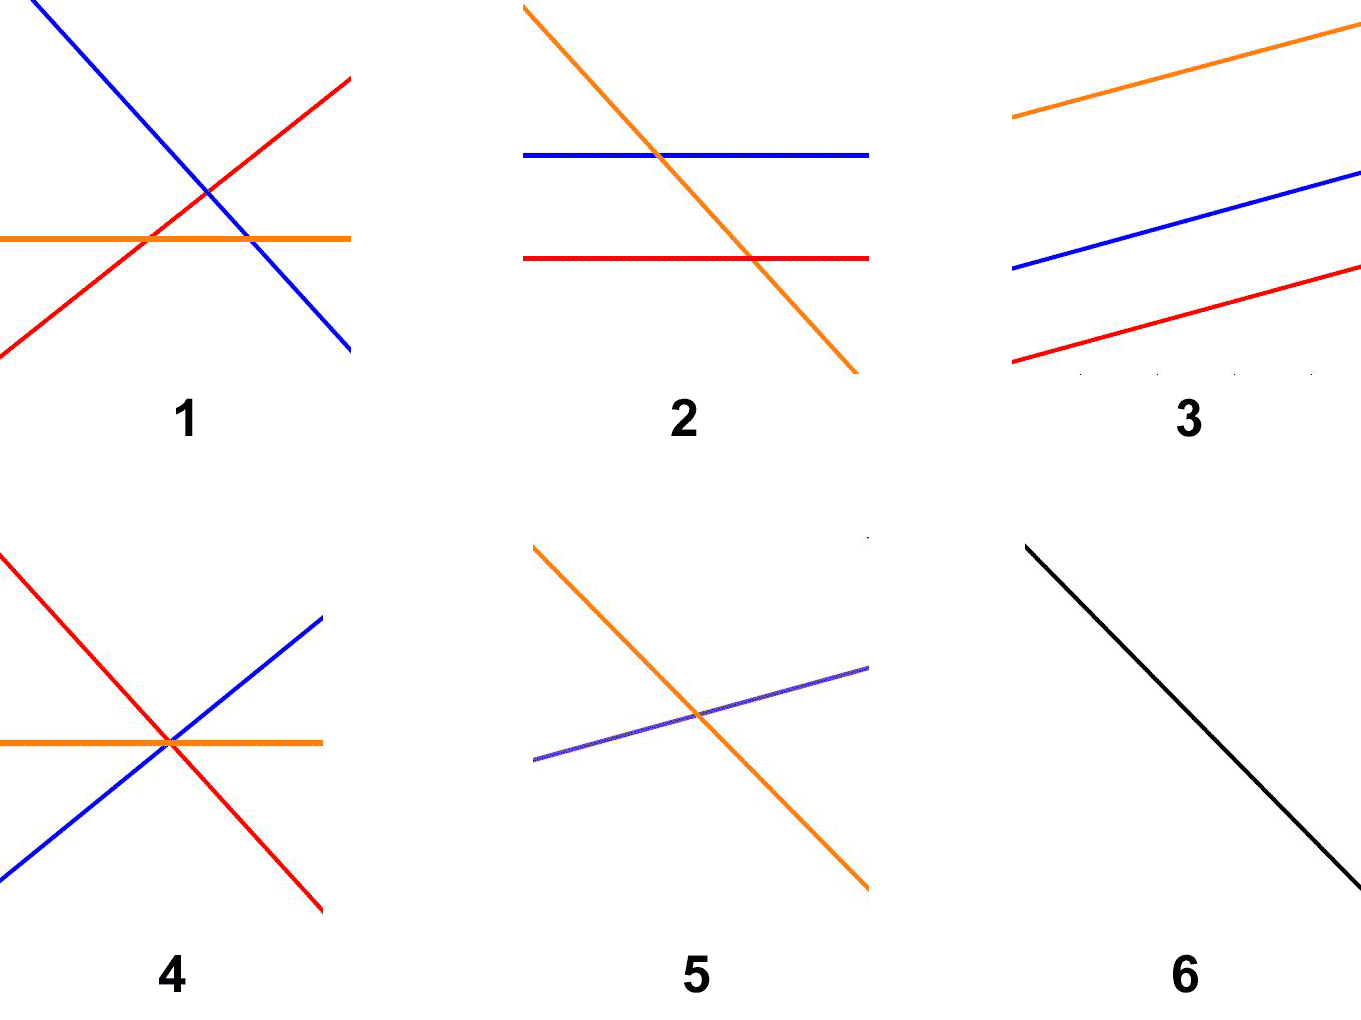
\includegraphics[width=0.8\textwidth]{6stregerien.png}
	\caption{De seks mulige løsningsstrukturer for tre ligninger med to ubekendte.} \label{tn2.figloes}
\end{figure}
I situation 2 er to af linjerne parallelle, og i situation 3 er alle tre linjer parallelle. Der er derfor ingen fælles punkter for alle de tre linjer i situationerne 1, 2 og 3. I situation 5 er to af linjerne sammenfaldende (blå og røde linje falder sammen i lilla linje). Der er derfor netop ét fælles punkt i situationerne 4 og 5. I situation 6 er alle tre linjer sammenfaldende (giver sort linje). Der er derfor i denne situation uendeligt mange fællespunkter.\\

Eksemplet med de tre ligninger med to ubekendte illustrerer den følgende sætning som følger af vores studium af løsningsmængder i det foregående afsnit, se sætningerne \ref{TN2.11c0}, \ref{TN2.11c} og \ref{TN2.11c2}:

\begin{theorem}[Bemærkning om antal løsninger]
Et lineært ligningssystem har enten ingen, eller én eller uendeligt mange løsninger. Andre muligheder findes ikke.
\end{theorem}

%%%%%%%%%%%%%%%%%%%%%%%%%%%%%%%%%%%%%%%%%%%%%%%%%%%%%%%%%%%%%%%%%%%%%%%%%%%%%%%%%
\section{Løsningsmængders lineære struktur} \label{TN2.afsnit.linstruk}
I dette afsnit vil vi gå lidt dybere ned i spørgsmålet om \textit{strukturen} af løsningsmængder for lineære ligningssystemer. Det er i særlig grad vigtigt at bemærke sammenhængen mellem løs\-nings\-mæng\-den for et inhomogent ligningssystem og løsningsmængden for \textit{det tilsvarende homogene ligningssystem}. Vi starter med at undersøge homogene ligningssystemer.

\subsection{Homogene ligningssystemers egenskaber}
Et homogent lineært ligningssystem af $m$ lineære ligninger med $n$ ubekendte skrives på formen
\begin{eqnalign}{rcrcrcrcl} \label{TN2.20}
a_{11}\cdot x_1 &+& a_{12}\cdot x_2 &+& \ldots &+& a_{1n}\cdot x_n &=& 0\\
a_{21}\cdot x_1 &+& a_{22}\cdot x_2 &+& \ldots &+& a_{2n}\cdot x_n &=& 0\\
 &&  &\vdots & && &&\\
a_{m1}\cdot x_1 &+& a_{m2}\cdot x_2 &+& \ldots &+& a_{mn}\cdot x_n &=& 0
\end{eqnalign}

I den følgende sætning beskriver vi en vigtig egenskab ved strukturen af løs\-nings\-mæng\-den for homogene lineære ligningssystemer.

\begin{theorem}[Løsninger til homogent lineært ligningssystem]\label{TN2.17}
Lad $L_{hom}$ betegne løsningsmængden for et homogent lineært ligningssystem. Så findes der mindst én løsning til systemet. Hvis
\begin{equation}
\mathbf x=(x_1,\,x_2,\,\ldots\,x_n)\quad \mathrm{og} \quad \mathbf y=(y_1,\,y_2,\,\ldots\,y_n)
\end{equation}
er to vilkårlige løsninger, og $k$ er et vilkårligt reelt tal, så vil både summen
\begin{equation}
\mathbf x + \mathbf y=(x_1+y_1,\,x_2+y_2,\,\ldots\,x_n+y_n)
\end{equation}
og produktet
\begin{equation}
k\cdot \mathbf x = (k\cdot x_1,\,k\cdot x_2,\,\ldots\,k\cdot x_n)
\end{equation}
tilhøre $L_{hom}$.
\end{theorem}

\begin{bevis}
En oplagt egenskab ved systemet (\ref{TN2.20}) er at $\rho(\mathbf A)= \rho(\mathbf T)$ (fordi højresiderne er lutter nuller). Systemet har derfor mindst én løsning - det følger af sætning \ref{TN2.11c}. Vi kan også straks finde en løsning, nemlig $0$-vektoren, $\mathbf 0 \in \mathbb R^n\,$. At den er en løsning fremgår jo af, at når vi erstatter alle de $n$ ubekendte i systemet med tallet $0$, så består systemet nemlig af $m$ ligninger af form $0=0$.\bs
Sætningen indeholder derudover to dele som bevises hver for sig:
\begin{enumerate}
\item
Hvis
\begin{equation}
a_{i1}x_1+a_{i2}x_2+\cdots + a_{in}x_n=0 \quad \textrm{for ethvert} \quad i=1,2,\ldots , m
\end{equation}
og
\begin{equation}
a_{i1}y_1+a_{i2}y_2+\cdots + a_{in}y_n=0 \quad \textrm{for ethvert} \quad i=1,2,\ldots , m
\end{equation}
så fås ved addition af de to ligninger og efterfølgende faktorisering med hensyn til koefficienterne
\begin{equation}
a_{i1}(x_1+y_1) + a_{i2}(x_2+y_2) + \cdots + a_{in}(x_n+y_n)=0 \quad \textrm{for ethvert} \quad i=1,2,\ldots , m
\end{equation}
hvilket viser at $\mathbf x + \mathbf y$ er en løsning.
\item
Hvis
\begin{equation}
a_{i1}x_1+a_{i2}x_2+\cdots + a_{in}x_n=0 \quad \textrm{for ethvert} \quad i=1,2,\ldots , m
\end{equation}
og $k$ er et vilkårligt reelt tal, så fås ved multiplikation på begge sider med $k$ og efterfølgende faktorisering med hensyn til koefficienterne
\begin{equation}
a_{i1}(k \cdot x_1)+a_{i2}(k \cdot x_2)+\cdots + a_{in}(k\cdot x_n)=0\quad \textrm{for ethvert}\quad i=1,2,\ldots,m
\end{equation}
hvilket viser at $k\cdot \mathbf x$ er en løsning.
\end{enumerate}
\end{bevis}

\begin{remark}
Hvis man tager et vilkårligt antal løsninger fra $L_{hom}$, ganger dem med vilkårlige konstanter og lægger disse produkter sammen, så vil denne såkaldte \ind{linearkombination}{linearkombination} af løsninger også selv være en løsning. Dette er en konsekvens af sætning \ref{TN2.17}. 
\end{remark}

%Det er interessant at studere sammenhængen mellem de her udviklede egenskaber for $L_{hom}$ og den løsningsstruktur for generelle lineære ligningssystemer med rang mindre end antal ubekendte, som vi nåede frem til ved hjælp af GaussJordan-elimination i metode \ref{TN2.19}:
%\begin{equation}
%\mathbf x=\mathbf x_0+t_1\,\mathbf v_1+t_2\,\mathbf v_2+\cdots+t_{n-k}\,\mathbf v_{n-k}\,.
%\end{equation}
%Høj\-re\-si\-der\-ne i et vilkårligt homogent ligningssystem består af lutter 0-er, og da disse 0-er ikke vil blive ændret ved de rækkeoperationer der fører frem til fuldstændigt reduceret form, vil $L_{hom}$ altid have begyndelsespunktet $\mathbf x_0=\mathbf 0$. Herved har vi (igen) set at 0-vektoren altid er en løsningsmulighed for et vilkårligt homogent lig\-ningssystem.\bs
%Vi kan derfor præcisere løsningsformlen for homogene systemer således:
%\begin{equation}\label{TN2.22}
%\mathbf x=t_1\,\mathbf v_1+t_2\,\mathbf v_2+\cdots+t_{n-k}\,\mathbf v_{n-k}\,.
%\end{equation}

%\begin{aha}
%Bemærk at sætning \ref{TN2.17} bekræftes af formlen (\ref{TN2.22}). Vælger man nemlig to vektorer på formen (\ref{TN2.22}), så kan deres sum (efter faktorisering) skrives på den selv samme form. Og det samme kan produktet af en konstant og en vektor på formen (\ref{TN2.22}).
%\end{aha}

\subsection{Struktursætningen} \label{TN2.afsnit.struktur}
Vi skal nu betragte en afgørende relation mellem et inhomogent lineært ligningssystem af formen 
\begin{eqnalign}{rcrcrcrcl}\label{TN2.23}
a_{11}\cdot x_1 &+& a_{12}\cdot x_2 &+& \ldots &+& a_{1n}\cdot x_n &=& b_1\\
a_{21}\cdot x_1 &+& a_{22}\cdot x_2 &+& \ldots &+& a_{2n}\cdot x_n &=& b_2\\
 &&  &\vdots & && &&\\
a_{m1}\cdot x_1 &+& a_{m2}\cdot x_2 &+& \ldots &+& a_{mn}\cdot x_n &=& b_m
\end{eqnalign}
og \textit{det tilhørende homogene lineære ligningssystem}, hvorved menes ligningerne (\ref{TN2.23}) efter at alle højresider $b_i$ er udskiftet med $0$. Løsningsmængden for det inhomogene ligningssystem kaldes $L_{inhom}$ og løsningsmængden for det tilhørende homogene ligningssystem for $L_{hom}$. 

\begin{theorem}[Struktursætningen]\label{TN2.23b}
Hvis der er fundet bare en enkelt løsning (en såkaldt \ind{partikulær løsning}{partikulær} løsning) $\mathbf x_0$ til et inhomogent lineært ligningssystem, så kan $L_{inhom}$ findes som summen af $\mathbf x_0$ og  $L_{hom}$.\bs
Der gælder med andre ord
\begin{equation}
L_{inhom}=\maengde{\mathbf x=\mathbf x_0+\mathbf y}{\mathbf y \in L_{hom}}.
\end{equation}
eller kort skrevet
\begin{equation}\label{TN2.24}
L_{inhom}=\mathbf x_0+L_{hom}.
\end{equation}
\end{theorem}

\begin{bevis}
Bemærk at sætningen rummer to påstande. Den ene er at summen af $\mathbf x_0$ og en vilkårlig vektor fra $L_{hom}$ tilhører $L_{inhom}$. Den anden er at en vilkårlig vektor fra $L_{inhom}$ kan skrives som summen af $\mathbf x_0$ og en vektor fra $L_{hom}$. Vi beviser de to påstande hver for sig:
\begin{enumerate}
\item
Antag $\mathbf y \in L_{hom}$. Vi ønsker at vise at 
\begin{equation}
\mathbf x=\mathbf x_0+\mathbf y=(x_{0_1}+y_1, x_{0_2}+y_2,\ldots ,x_{0_n}+y_n) \in L_{inhom}.
\end{equation}
Da
\begin{equation}
a_{i1}x_{0_1}+a_{i2}x_{0_2}+ \cdots + a_{in}x_{0_n}=b_i \quad \textrm{for ethvert}\quad i=1,2,\ldots,m
\end{equation}
og
\begin{equation}
a_{i1}y_{1}+a_{i2}y_{2}+ \cdots + a_{in}y_{n}=0 \quad \textrm{for ethvert}\quad i=1,2,\ldots,m
\end{equation}
så fås ved addition af de to ligninger og efterfølgende faktorisering med hensyn til koefficienterne
\begin{equation}
a_{i1}(x_{0_1}+y_1) + \cdots + a_{in}(x_{0_n}+y_n) = b_i \quad \textrm{for ethvert} \quad i=1,2,\ldots,m
\end{equation}
hvilket viser det ønskede.
\item
Antag at $\mathbf x \in L_{inhom}$. Vi ønsker at vise at der findes en vektor  $\mathbf y \in L_{hom}$ der opfylder at
\begin{equation}
\mathbf x=\mathbf x_0+\mathbf y.
\end{equation}
Da både  $\mathbf x$ og  $\mathbf x_0$ tilhører $L_{inhom}$ gælder at
\begin{equation}
a_{i1}x_{1}+ a_{i2}x_{2}+\cdots + a_{in}x_{n}=b_i \quad \textrm{for ethvert} \quad i=1,2,\ldots,m
\end{equation}
og
\begin{equation}
a_{i1}x_{0_1}+a_{i2}x_{0_2}+\cdots + a_{in}x_{0_n}=b_i \quad \textrm{for ethvert} \quad i=1,2,\ldots,m
\end{equation}
Når vi fra den øverste ligning trækker den nederste, får vi efter faktorisering
\begin{equation}
a_{i1}(x_1-x_{0_1})+\cdots + a_{in}(x_n-x_{0_n})=0 \quad \textrm{for ethvert} \quad i=1,2,\ldots,m
\end{equation}
hvilket viser at den vektor $\mathbf y$ som defineres ved $\mathbf y=\mathbf x -\mathbf x_0$, tilhører $L_{hom}$ og opfylder det ønskede: $\mathbf x=\mathbf x_0+\mathbf y$. 
\end{enumerate}
\end{bevis}

%Lad os perspektivere denne sætning ved hjælp af løsningsstrukturen for generelle lineære ligningssystemer med rang mindre end antal ubekendte, som vi nåede frem til ved hjælp af \tref{TN2.19}{metode}:
%\begin{equation}\label{TN2.24b}
%\mathbf x=\mathbf x_0+t_1\,\mathbf v_1+t_2\,\mathbf v_2+\cdots+t_{n-k}\,\mathbf v_{n-k}\,.
%\end{equation}
%Ved at sætte alle de frie parametre $t_1,t_2,\ldots,t_n$ lig med 0, ses det at $\mathbf x_0$ er en partikulær løsning til det givne ligningssystem. Linearkombinationen $t_1\,\mathbf v_1+t_2\,\mathbf v_2+\cdots+t_{n-k}\,\mathbf v_{n-k}$ er løsningsmængden for det tilsvarende homogene ligningssystem, se ligning (\ref{TN2.22}).

%\begin{aha}
%Bemærk at sætning \ref{TN2.23b} bekræftes af formlen (\ref{TN2.24b}) i den forstand, at der i hvert fald findes ét begyndelsespunkt $\mathbf x_0$ således at $L_{inhom}=\mathbf x_0+L_{hom}$, nemlig det begyndelsespunkt der fremkommer af GaussJordan-eliminationen. Men sætning \ref{TN2.23b} går et skridt videre idet den siger at en vilkårlig løsning til det inhomogene system kan benyttes som begyndelsespunkt.
%\end{aha}

\end{document} 
\begin{summary}\label{TN2.25}
Vi ser på lineære ligningssystemer, indfører metoder til at beskrive og løse dem, og vi analyserer løsningsmængdernes struktur.

\begin{itemize}
\item
Et \ind{lineært ligningssystem}{lineært ligningssystem} bestående af $m$ lineære ligninger med $n$ ubekendte skrives på formen
\begin{eqnalign}{rcrcrcrcl} \label{TN2.4}
a_{11}\cdot x_1 &+& a_{12}\cdot x_2 &+& \ldots &+& a_{1n}\cdot x_n &=& b_1\\
a_{21}\cdot x_1 &+& a_{22}\cdot x_2 &+& \ldots &+& a_{2n}\cdot x_n &=& b_2\\
 &&  &\vdots & && &&\\
a_{m1}\cdot x_1 &+& a_{m2}\cdot x_2 &+& \ldots &+& a_{mn}\cdot x_n &=& b_m
\end{eqnalign}
\item
Ligningssystemet kan have ingen løsninger, netop én løsning eller uendeligt mange løsninger, andre muligheder findes ikke.
\item
Ligningssystemets koefficientmatrix $\mathbf A$, dets højreside $\mathbf b$ og dets totalmatrix $\mathbf T$ defineres ved
\begin{equation}
\mathbf{A}=
\begin{matr}{cccc}
 a_{11}&a_{12}&\cdots & a_{1n} \\
 a_{21}&a_{22}&\cdots & a_{2n} \\
 \vdots&\vdots&&\vdots\\
 a_{m1}&a_{m2}&\cdots&a_{mn}
\end{matr},\,
\mathbf{b}=
\begin{matr}{c}
b_1\\ b_2 \\ \vdots\\b_m
\end{matr} \;\mathrm{og}\;
\mathbf{T}=
\begin{matr}{cccc|c}
 a_{11}&a_{12}&\cdots&a_{1n} & b_1\\
  a_{21}&a_{22}&\cdots&a_{2n} & b_2\\
  \vdots&\vdots&&\vdots\\
 a_{m1}&a_{m2}&\cdots&a_{mn} & b_m
\end{matr}. \nonumber
\end{equation}
\item
Ved hjælp af tre typer af \ind{rækkeoperationer}{rækkeoperationer} kan ligningssystemet reduceres fuldstændigt, svarende til at $\mathbf T$ omformes til en \textit{trappematrix} trap$(\mathbf T)$. Ligningssystemets (og trappematricens) \textit{rang} er antallet af ikke $0$-rækker i trap$(\mathbf T)$. 
\item
Hvis trap$(\mathbf T)$ indeholder en række af formen $ \begin{matr}{cccc|c} 0 & 0 & \cdots & 0 & 1 \end{matr} $ har lig\-nings\-sy\-stem\-et ingen løsninger, i modsat fald kan løsningsmængden skrives på formen:
\begin{equation}
\mathbf x=\mathbf x_0+t_1\,\mathbf v_1+t_2\,\mathbf v_2+\cdots+t_{n-k}\,\mathbf v_{n-k}\,.
\end{equation}
hvor $n$ er antallet af ubekendte, og $\,k\leq n\,$ er systemets rang. Hvis lig\-nings\-sy\-stem\-ets er inhomogent, er \textit{begyndelsespunktet} $\mathbf x_0\neq \bold{0}$, og løsningsmængden til det tilsvarende homogene ligningssystem er da alle tænkelige \ind{linearkombination}{linearkombinationer} af de $(n-k)$ \textit{retningsvektorer}:
\begin{equation}
\mathbf x=t_1\,\mathbf v_1+t_2\,\mathbf v_2+\cdots+t_{n-k}\,\mathbf v_{n-k}\,,
\end{equation}
hvor $t_1,t_2,\ldots,t_{n-k}\in \mathbb R\,$.
\end{itemize}

\end{summary}









%%%%%%%%%%%%%%%%%%%%%%%%%%%%%%%%%%%%%%%%%%%%%
%%%%%%%%%%%%%%%%%%%%%%%%%%%%%%%%%%%%%%%%%%%%%
%%% HER SKAL DU STOPPE MED AT SKRIVE %%%%%%%%
%%%%%%%%%%%%%%%%%%%%%%%%%%%%%%%%%%%%%%%%%%%%%
%%%%%%%%%%%%%%%%%%%%%%%%%%%%%%%%%%%%%%%%%%%%%


\end{document} 